\documentclass[11pt,a4paper]{article}
\usepackage[T1]{fontenc}
\usepackage[utf8]{inputenc}
\usepackage[polish]{babel}
\usepackage{mathptmx}
\usepackage[margin=2.5cm]{geometry}
\usepackage{amsmath,graphicx,booktabs,array,tabularx,float,caption,microtype}
\usepackage{tikz}
\usetikzlibrary{arrows.meta}
\usepackage[hidelinks]{hyperref}
\setlength{\parindent}{0pt}
\setlength{\parskip}{4pt}
\setlength{\tabcolsep}{6pt}
\renewcommand{\arraystretch}{1.12}
\captionsetup{font=small,labelfont=bf}
\hypersetup{
  pdftitle={SIGK -- Projekt 1: Odszumianie i deblurring},
  pdfauthor={Aleksandra Buczma; Aleksandra Samsel},
  pdfsubject={Zespół Olé, zadania 2.2 i 2.3}
}

% Generated from verified final 100-image evaluation; do not copy holdout values here.
\newif\ifFinalResultsReady
\FinalResultsReadytrue
\newcommand{\FinalSampleCount}{100}
\newcommand{\FinalNoisyPSNRLow}{40.0746}
\newcommand{\FinalNoisySSIMLow}{0.97222}
\newcommand{\FinalNoisyLPIPSLow}{0.00877}
\newcommand{\FinalBilateralPSNRLow}{40.9267}
\newcommand{\FinalBilateralSSIMLow}{0.98645}
\newcommand{\FinalBilateralLPIPSLow}{0.00566}
\newcommand{\FinalUNetPSNRLow}{42.5576}
\newcommand{\FinalUNetSSIMLow}{0.99047}
\newcommand{\FinalUNetLPIPSLow}{0.00305}
\newcommand{\FinalNoisyPSNRHigh}{30.5998}
\newcommand{\FinalNoisySSIMHigh}{0.83740}
\newcommand{\FinalNoisyLPIPSHigh}{0.06936}
\newcommand{\FinalBilateralPSNRHigh}{33.5347}
\newcommand{\FinalBilateralSSIMHigh}{0.93368}
\newcommand{\FinalBilateralLPIPSHigh}{0.03819}
\newcommand{\FinalUNetPSNRHigh}{34.3689}
\newcommand{\FinalUNetSSIMHigh}{0.93792}
\newcommand{\FinalUNetLPIPSHigh}{0.03987}
\newcommand{\JointBestEpoch}{27}
\newcommand{\JointCheckpointHash}{9aa445241b9ecec8b84fb0c0420272ac6206583e2f9ca5174ce741769eba04a9}
\newcommand{\JointRunLabel}{unet\_joint\_balanced\_v5}
\newcommand{\FinalLowPSNRGain}{+1.6309}
\newcommand{\FinalLowAllMetrics}{TAK}
\newcommand{\FinalHighPSNRGain}{+0.8342}
\newcommand{\FinalHighAllMetrics}{NIE}
\newcommand{\FinalOverallConclusion}{Wspólny checkpoint przewyższył filtr bilateralny na wszystkich trzech średnich metrykach dla poziomu szumu 0.01. Przy drugim poziomie wyniki są mieszane; nie uzyskano przewagi na wszystkich trzech metrykach jednocześnie przy obu poziomach.}


\newcommand{\columnlabels}{%
  \begin{tabularx}{\linewidth}{@{}*{4}{>{\centering\arraybackslash}X}@{}}
    Obraz zaszumiony & Filtr bilateralny & Residual U-Net & Obraz referencyjny
  \end{tabularx}\par\vspace{3pt}}
\newcommand{\imagerow}[2]{%
  {\small\textbf{DIV2K #2}}\par\vspace{2pt}
  \includegraphics[width=0.242\linewidth]{images/denoising/noisy_#1_#2.png}\hfill
  \includegraphics[width=0.242\linewidth]{images/denoising/bilateral_#1_#2.png}\hfill
  \includegraphics[width=0.242\linewidth]{images/denoising/unet_#1_#2.png}\hfill
  \includegraphics[width=0.242\linewidth]{images/denoising/clean_#2.png}\par\vspace{7pt}}
\newcommand{\deblurexperiment}[1]{\par\vspace{2pt}{\bfseries #1}\par}

\begin{document}
\begin{center}
  {\LARGE\bfseries SIGK -- Projekt 1}\par
  \vspace{4pt}
  {\large Odszumianie i deblurring}\par
  \vspace{4pt}
  \textbf{Zespół Olé}\quad Aleksandra Buczma, Aleksandra Samsel
\end{center}

\begingroup\small

\section*{Architektura sieci neuronowej}
W obu zadaniach zastosowano tę samą architekturę residual U-Net w PyTorch,
ucząc oddzielne wagi. Wejściem jest zaszumiony lub rozmyty obraz RGB,
a wyjściem jego rekonstrukcja. Oba tensory mają rozmiar
$B\times3\times256\times256$, gdzie $B$ oznacza liczbę obrazów w partii.

Enkoder ma trzy bloki \texttt{DoubleConv}, każdy z dwiema konwolucjami
$3\times3$ i aktywacją ReLU po każdej z nich. Padding równy 1 zachowuje
rozmiar obrazu. Max pooling $2\times2$ zmniejsza rozdzielczość, a liczba
kanałów rośnie: $16\rightarrow32\rightarrow64\rightarrow128$.
Ostatni poziom, tzw. bottleneck, ma rozmiar $128\times32\times32$.

Dekoder trzykrotnie powiększa mapy cech interpolacją biliniową.
Każdy \texttt{UpBlock} zawiera konwolucję redukującą kanały z ReLU,
konkatenację cech z enkodera oraz \texttt{DoubleConv}.
Połączenia te pomagają zachować szczegóły obrazu.
Końcowa konwolucja $1\times1$ daje trzykanałową poprawkę $F_\theta(x)$,
dodawaną do wejścia: $\hat{y}=x+F_\theta(x)$.
Sieć ma 535\,827 parametrów, 18 konwolucji i 17 aktywacji ReLU;
nie stosuje batch normalization, dropout ani końcowej funkcji aktywacji.

\begin{figure}[H]
\centering

\begin{tikzpicture}[
  font=\scriptsize,
  block/.style={draw,rounded corners=2pt,align=center,text width=3.7cm,
                minimum height=0.87cm,inner sep=3pt,line width=0.6pt},
  enc/.style={block,draw=blue!55!black,fill=blue!7},
  dec/.style={block,draw=teal!65!black,fill=teal!8},
  io/.style={block,text width=3.1cm,draw=black!60,fill=black!3},
  flow/.style={-{Latex[length=2mm]},line width=0.7pt,draw=black!75},
  skip/.style={flow,dashed,draw=orange!65!black},
  note/.style={font=\tiny,fill=white,inner sep=1.5pt}
]
\node[io] (input) at (-4,2.35)
  {\textbf{Wejście $x$: obraz RGB}\\$3\times256\times256$};
\node[enc] (e1) at (-4,0)
  {\textbf{E1: DoubleConv ($3\rightarrow16$)}\\$16\times256\times256$};
\node[enc] (e2) at (-4,-1.4)
  {\textbf{E2: DoubleConv ($16\rightarrow32$)}\\$32\times128\times128$};
\node[enc] (e3) at (-4,-2.8)
  {\textbf{E3: DoubleConv ($32\rightarrow64$)}\\$64\times64\times64$};
\node[block,draw=violet!60!black,fill=violet!8] (b) at (0,-4.2)
  {\textbf{B: DoubleConv ($64\rightarrow128$)}\\$128\times32\times32$};
\node[dec] (d3) at (4,-2.8)
  {\textbf{D3: UpBlock ($128\rightarrow64$)}\\$64\times64\times64$};
\node[dec] (d2) at (4,-1.4)
  {\textbf{D2: UpBlock ($64\rightarrow32$)}\\$32\times128\times128$};
\node[dec] (d1) at (4,0)
  {\textbf{D1: UpBlock ($32\rightarrow16$)}\\$16\times256\times256$};
\node[block,text width=3.1cm,draw=teal!65!black,fill=teal!8] (head) at (0.7,1.15)
  {\textbf{Conv $1\times1$ ($16\rightarrow3$)}\\$F_\theta(x):\ 3\times256\times256$};
\node[circle,draw,line width=0.7pt,minimum size=0.45cm,inner sep=0pt] (sum) at (0.7,2.35) {$+$};
\node[io] (output) at (4,2.35)
  {\textbf{Wyjście $\hat{y}$: rekonstrukcja}\\$3\times256\times256$};

\draw[flow] (input.south) -- (e1.north);
\draw[flow] (e1.south) -- node[note,left]{MaxPool $2\times2$} (e2.north);
\draw[flow] (e2.south) -- node[note,left]{MaxPool $2\times2$} (e3.north);
\draw[flow] (e3.south) |- node[note,pos=0.75,above]{MaxPool $2\times2$} (b.west);
\draw[flow] (b.east) -| (d3.south);
\draw[flow] (d3.north) -- (d2.south);
\draw[flow] (d2.north) -- (d1.south);
\draw[flow] (d1.north) |- (head.east);
\draw[flow] (head.north) -- (sum.south);
\draw[flow] (input.east) -- node[note,above]{połączenie rezydualne} (sum.west);
\draw[flow] (sum.east) -- (output.west);
\draw[skip] (e1.east) -- node[note,above]{concat: $16+16=32$} (d1.west);
\draw[skip] (e2.east) -- node[note,above]{concat: $32+32=64$} (d2.west);
\draw[skip] (e3.east) -- node[note,above]{concat: $64+64=128$} (d3.west);
\end{tikzpicture}

\caption{Residual U-Net wspólny dla obu zadań. Wymiary zapisano jako
$C\times H\times W$, pomijając wymiar partii $B$.
Linie przerywane oznaczają konkatenację z cechami enkodera;
podano liczbę kanałów po połączeniu.}
\end{figure}


\section*{Dane}
Wykorzystano DIV2K: obrazy RGB o rozmiarze $256\times256$ i wartościach
w $[0,1]$. Podziały danych i trening dobrano osobno. Skalowanie wykonano
interpolacją bicubic z Pillow w części 2.2 oraz \texttt{INTER\_AREA}
z OpenCV w części 2.3.


\begingroup
\section*{Metryki ewaluacyjne}
\begin{itemize}
\item \textbf{PSNR (dB)} --- miara błędu pikselowego, im wyższa wartość, tym lepiej.
\item \textbf{SSIM} --- podobieństwo strukturalne (zakres 0--1), im wyżej, tym lepiej.
\item \textbf{LPIPS} --- percepcyjna odległość między obrazami, im niżej, tym lepiej; lepiej niż PSNR/SSIM odzwierciedla ludzką ocenę jakości obrazu.
\end{itemize}
\endgroup

\endgroup


\clearpage
\section*{2.2 Odszumianie}
Do uczenia użyto 720 obrazów, do strojenia 80, a do końcowego porównania
100 publicznych obrazów walidacyjnych. Publiczna walidacja zastępuje ukryty
oficjalny test, którego czyste obrazy nie są dostępne. Dodawano szum gaussowski
o odchyleniu standardowym $\sigma=0.01$ lub $0.03$, ograniczając wynik do $[0,1]$.

\subsection*{Funkcja straty}
Po wstępnym uczeniu z MSE model dostrajano przez 30 epok optymalizatorem Adam,
z learning rate $10^{-4}$ i partiami po 2 czyste obrazy. Każdy obraz miał
obie zaszumione wersje. Strata równoważyła poziomy szumu:
\[
\mathcal{L}=\frac{1}{2}\frac{\mathrm{MSE}_{0.01}}{0.01^2}
           +\frac{1}{2}\frac{\mathrm{MSE}_{0.03}}{0.03^2}.
\]
MSE oznacza średni błąd kwadratowy między wyjściem sieci a czystym obrazem.
Dzielenie przez wariancję szumu równoważy udział obu poziomów w uczeniu.
Wybrano wagi z epoki 27 na podstawie wyników na 80 obrazach do strojenia.

\subsection*{Wyniki}
Porównano sieć z filtrem bilateralnym scikit-image na tych samych zaszumionych
obrazach. Parametry filtra dobrano na zbiorze do strojenia:
\texttt{sigma\_color} $0.005/0.015$, \texttt{sigma\_spatial=3},
\texttt{mode='reflect'}. PSNR i SSIM powinny być wyższe, a LPIPS niższy.
Metryki obliczano dla każdego obrazu, po ograniczeniu wyjścia do $[0,1]$,
a następnie uśredniano osobno dla obu poziomów szumu. LPIPS wykorzystuje AlexNet.

\begin{table}[H]
\centering\small
\begin{tabular}{@{}clrrr@{}}
\toprule
$\sigma$ & Metoda & PSNR [dB] $\uparrow$ & SSIM $\uparrow$ & LPIPS $\downarrow$ \\
\midrule
0.01 & Obraz zaszumiony & \FinalNoisyPSNRLow & \FinalNoisySSIMLow & \FinalNoisyLPIPSLow \\
0.01 & Filtr bilateralny & \FinalBilateralPSNRLow & \FinalBilateralSSIMLow & \FinalBilateralLPIPSLow \\
0.01 & Residual U-Net & \textbf{\FinalUNetPSNRLow} & \textbf{\FinalUNetSSIMLow} & \textbf{\FinalUNetLPIPSLow} \\
\midrule
0.03 & Obraz zaszumiony & \FinalNoisyPSNRHigh & \FinalNoisySSIMHigh & \FinalNoisyLPIPSHigh \\
0.03 & Filtr bilateralny & \FinalBilateralPSNRHigh & \FinalBilateralSSIMHigh & \textbf{\FinalBilateralLPIPSHigh} \\
0.03 & Residual U-Net & \textbf{\FinalUNetPSNRHigh} & \textbf{\FinalUNetSSIMHigh} & \FinalUNetLPIPSHigh \\
\bottomrule
\end{tabular}
\caption{Średnie wyniki na 100 publicznych obrazach walidacyjnych DIV2K.
Pogrubiono najlepszy wynik dla każdej metryki i poziomu szumu.}
\end{table}

\clearpage
\subsection*{Porównanie obrazów}
\subsubsection*{Szum \texorpdfstring{$\sigma=0.01$}{sigma=0.01}}
\begin{figure}[H]
\centering
\columnlabels
\imagerow{sigma001}{0845}
\imagerow{sigma001}{0876}
\imagerow{sigma001}{0898}
\caption{Przykłady dla niskiego szumu. Wszystkie panele mają rozdzielczość
$256\times256$, a sieć i filtr otrzymały identyczne zaszumione wejścia.}
\end{figure}
Przy niskim szumie różnice wizualne są subtelne. Sieć zachowuje krawędzie
budynków i kontury kwiatów; średnie metryki wskazują poprawę względem filtra.

\clearpage
\subsubsection*{Szum \texorpdfstring{$\sigma=0.03$}{sigma=0.03}}
\begin{figure}[H]
\centering
\columnlabels
\imagerow{sigma003}{0845}
\imagerow{sigma003}{0876}
\imagerow{sigma003}{0898}
\caption{Te same obrazy przy wyższym szumie. Oba poziomy obsługuje identyczny
zestaw wag U-Net. Przykłady wybrano według treści, przed poznaniem wyniku treningu.}
\end{figure}
Na niebie obrazu 0845 i niebieskim tle 0898 po zastosowaniu sieci pozostaje
widoczne drobne ziarno, które filtr bilateralny usuwa skuteczniej.
Dla obrazu mostu 0876 U-Net uzyskuje lepsze wszystkie trzy metryki.
Pokazuje to, że skuteczność zależy także od treści obrazu.
\subsection*{Wnioski}
Dla $\sigma=0.01$ U-Net jest lepszy od filtra we wszystkich trzech metrykach.
Dla $\sigma=0.03$ poprawia PSNR i SSIM, ale LPIPS jest gorszy o około $4.4\%$.
Jeden model działa więc skutecznie na obu poziomach, jednak nie przewyższa
filtra w każdej metryce. Na gładkim tle części obrazów przy wyższym szumie
pozostają zakłócenia; przedstawione przykłady pokazują zarówno dobre,
jak i słabsze rekonstrukcje.

{\footnotesize\textbf{Źródła:}
\href{https://arxiv.org/abs/1505.04597}{U-Net (Ronneberger i in., 2015)};
\href{https://data.vision.ee.ethz.ch/cvl/DIV2K/}{DIV2K};
\href{https://arxiv.org/abs/1801.03924}{LPIPS (Zhang i in., 2018)}.}


\begingroup\small
\setlength{\intextsep}{4pt}
\setlength{\topsep}{3pt}
\captionsetup{skip=3pt}
\clearpage
\section*{2.3 Deblurring}
\subsection*{1. Baseline}
Jako punkt odniesienia (baseline) zastosowano klasyczną, nieuczoną metodę dekonwolucji --- algorytm Richardsona-Lucy'ego, który odtwarza ostry obraz na podstawie znanego kształtu rozmycia (tzw. PSF).

\subsection*{2. Funkcja straty}
Model trenowano, minimalizując sumę straty pikselowej (różnica wartości pikseli między predykcją a oryginalnym ostrym obrazem) oraz straty percepcyjnej opartej na cechach z sieci VGG16, która premiuje podobieństwo \textquotedbl{}wizualne\textquotedbl{} obrazów, a nie tylko identyczność pikseli.

\subsection*{3. Eksperymenty}
Model wytrenowano na rozmyciu gaussowskim o dwóch konfiguracjach: jądro 3x3 (\ensuremath{\sigma}=1.0) oraz jądro 5x5 (\ensuremath{\sigma}=1.5). Następnie, bez żadnego dodatkowego treningu, ten sam model przetestowano na szerszym zakresie siły rozmycia, aby sprawdzić jego zdolność do generalizacji. Dla każdej konfiguracji porównano metodę klasyczną (Richardson-Lucy) z siecią neuronową.

\subsubsection*{3.1 Jądro rozmycia 3x3}
\noindent\begin{minipage}{\linewidth}
\deblurexperiment{Eksperyment: \ensuremath{\sigma} = 0.5 (rozmycie słabsze niż treningowe)}
\begin{center}
\begin{tabular}{@{}lrrr@{}}
\toprule
Metoda & PSNR (dB) & SSIM & LPIPS \\
\midrule
Richardson-Lucy & 52.78 & 0.999 & 0.0003 \\
Sieć neuronowa & 23.40 & 0.843 & 0.255 \\
\bottomrule
\end{tabular}
\end{center}
\begin{center}
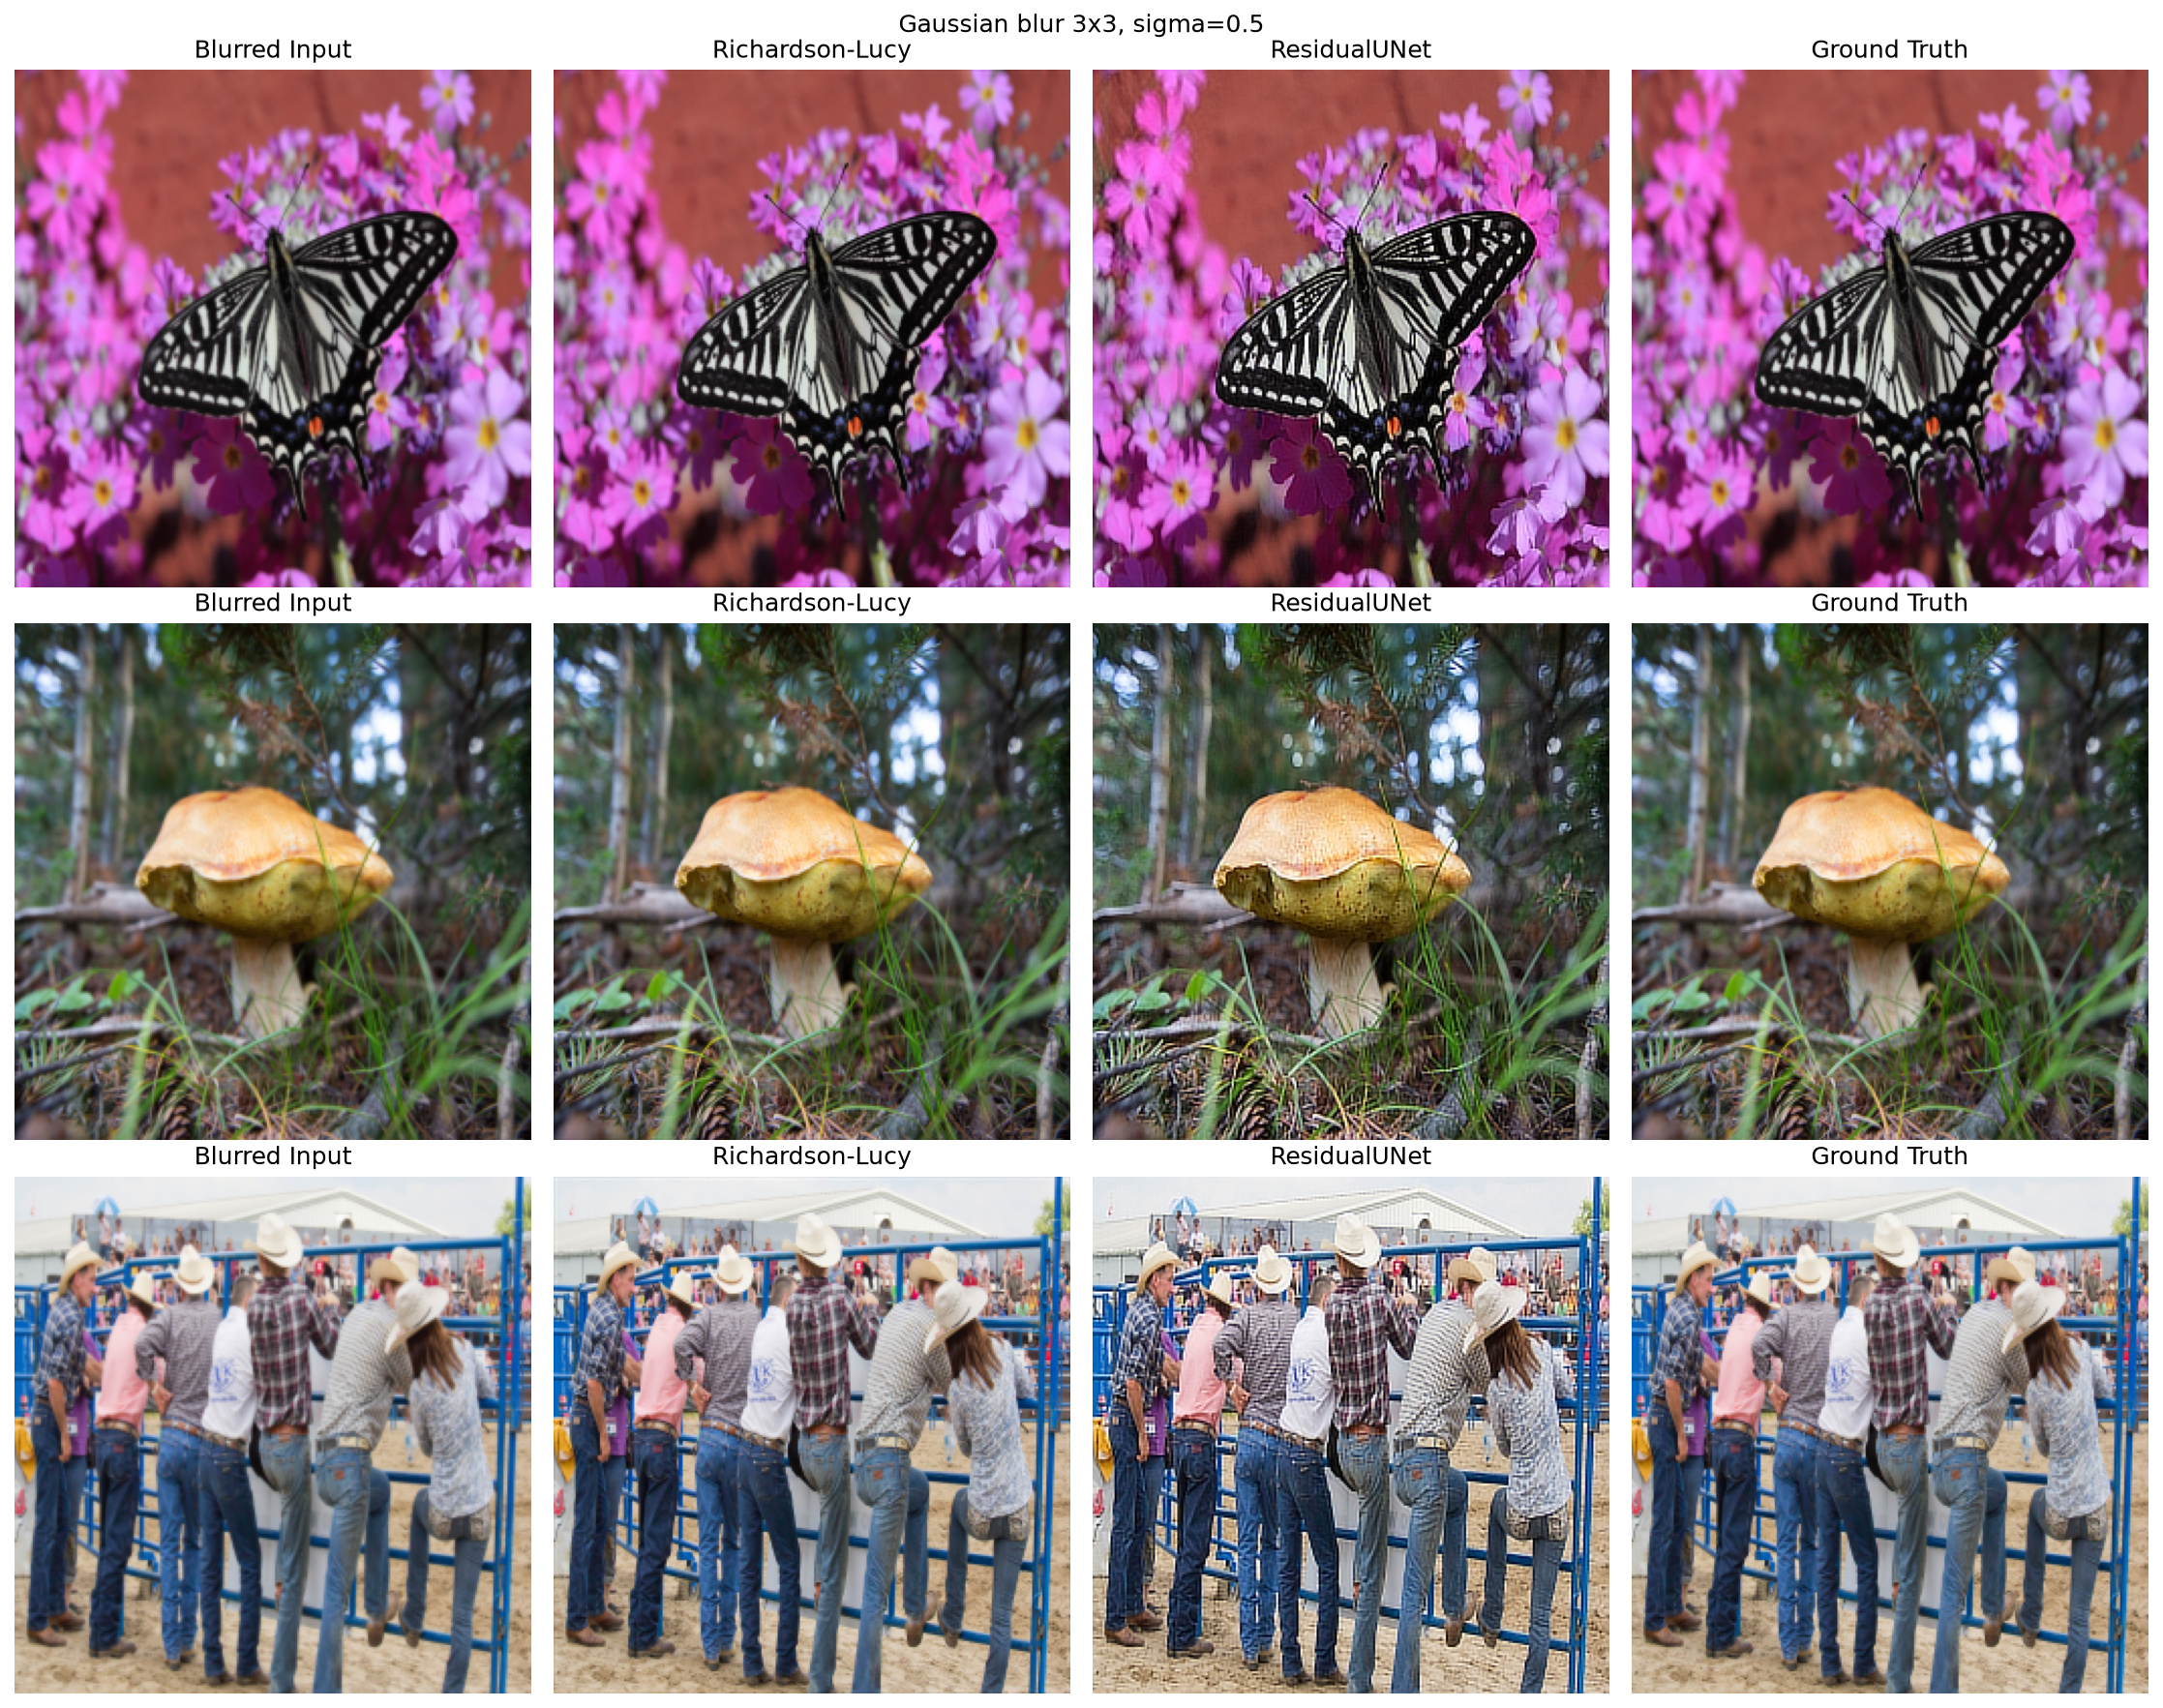
\includegraphics[width=0.67\linewidth]{images/deblurring_display/examples_k3_s0.5.jpg}\par
{\footnotesize Przykład \ensuremath{\sigma}=0.5, jądro 3x3}
\end{center}
\end{minipage}\par\vspace{5pt}
\noindent\begin{minipage}{\linewidth}
\deblurexperiment{Eksperyment: \ensuremath{\sigma} = 0.8 (rozmycie słabsze niż treningowe)}
\begin{center}
\begin{tabular}{@{}lrrr@{}}
\toprule
Metoda & PSNR (dB) & SSIM & LPIPS \\
\midrule
Richardson-Lucy & 22.92 & 0.935 & 0.111 \\
Sieć neuronowa & 33.33 & 0.970 & 0.014 \\
\bottomrule
\end{tabular}
\end{center}
\begin{center}
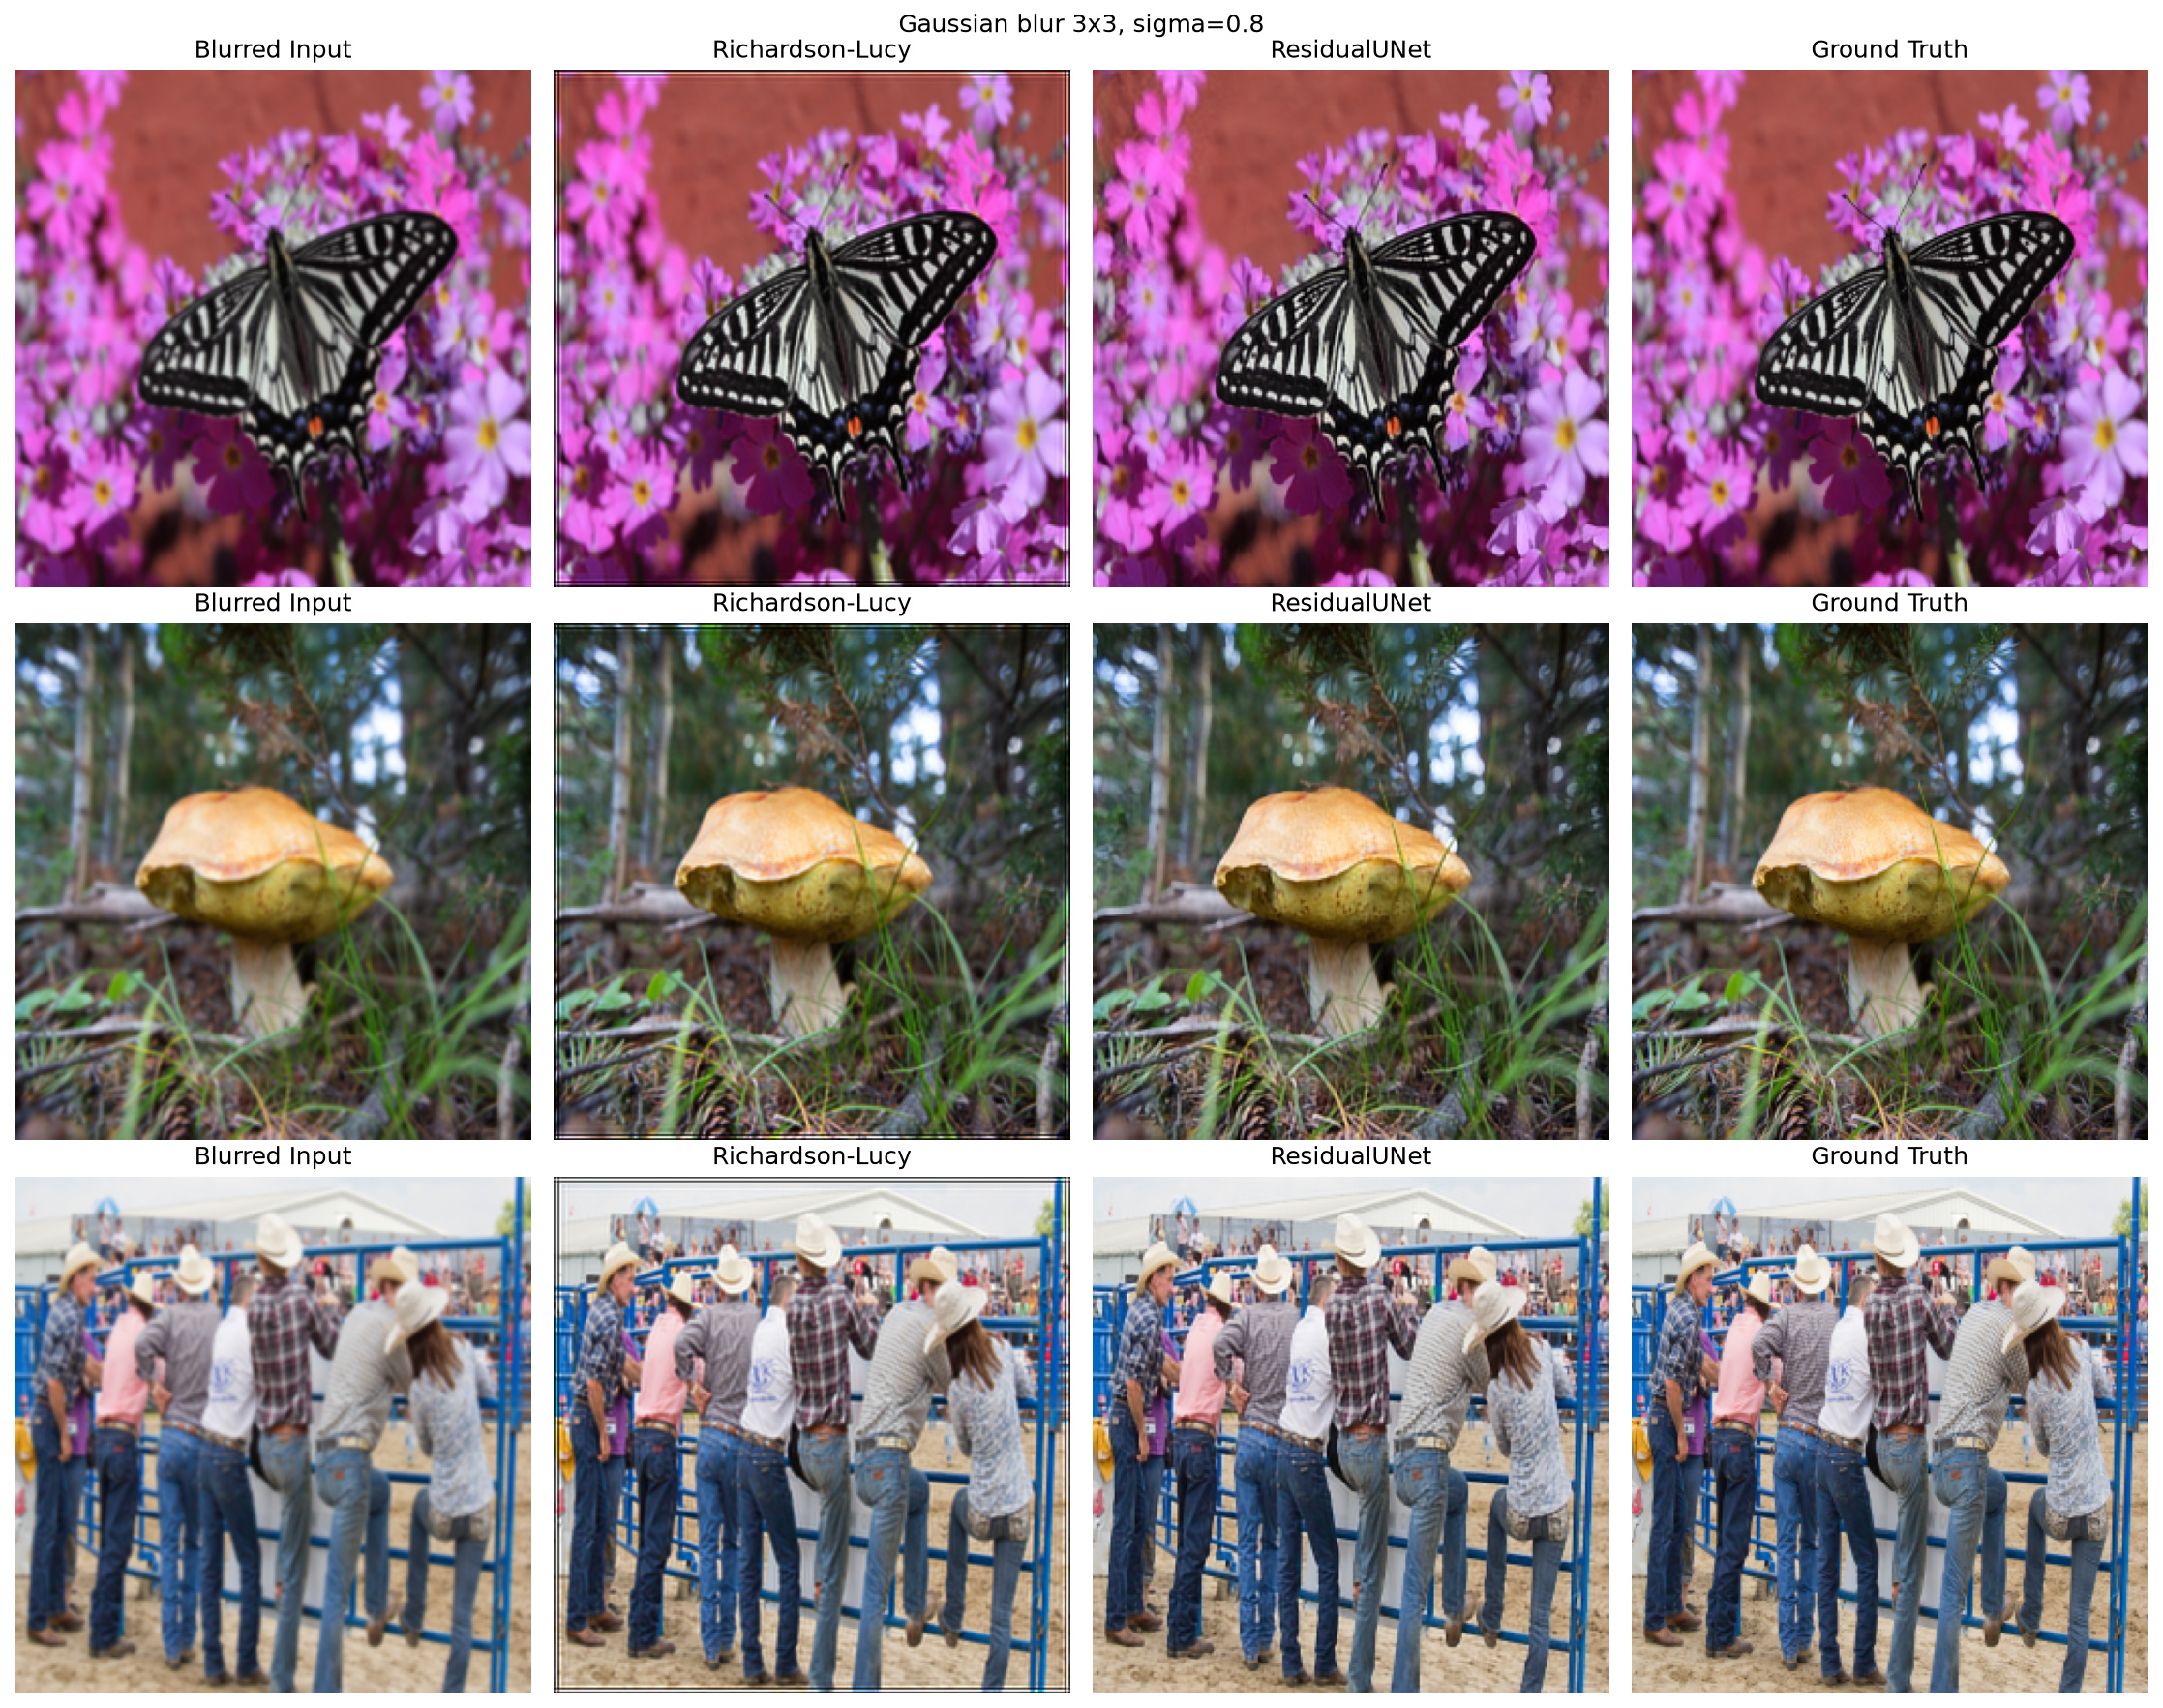
\includegraphics[width=0.67\linewidth]{images/deblurring_display/examples_k3_s0.8.jpg}\par
{\footnotesize Przykład \ensuremath{\sigma}=0.8, jądro 3x3}
\end{center}
\end{minipage}\par\vspace{5pt}
\noindent\begin{minipage}{\linewidth}
\deblurexperiment{Eksperyment: \ensuremath{\sigma} = 1.0 (siła rozmycia użyta w treningu)}
\begin{center}
\begin{tabular}{@{}lrrr@{}}
\toprule
Metoda & PSNR (dB) & SSIM & LPIPS \\
\midrule
Richardson-Lucy & 20.88 & 0.908 & 0.185 \\
Sieć neuronowa & 30.07 & 0.933 & 0.031 \\
\bottomrule
\end{tabular}
\end{center}
\begin{center}
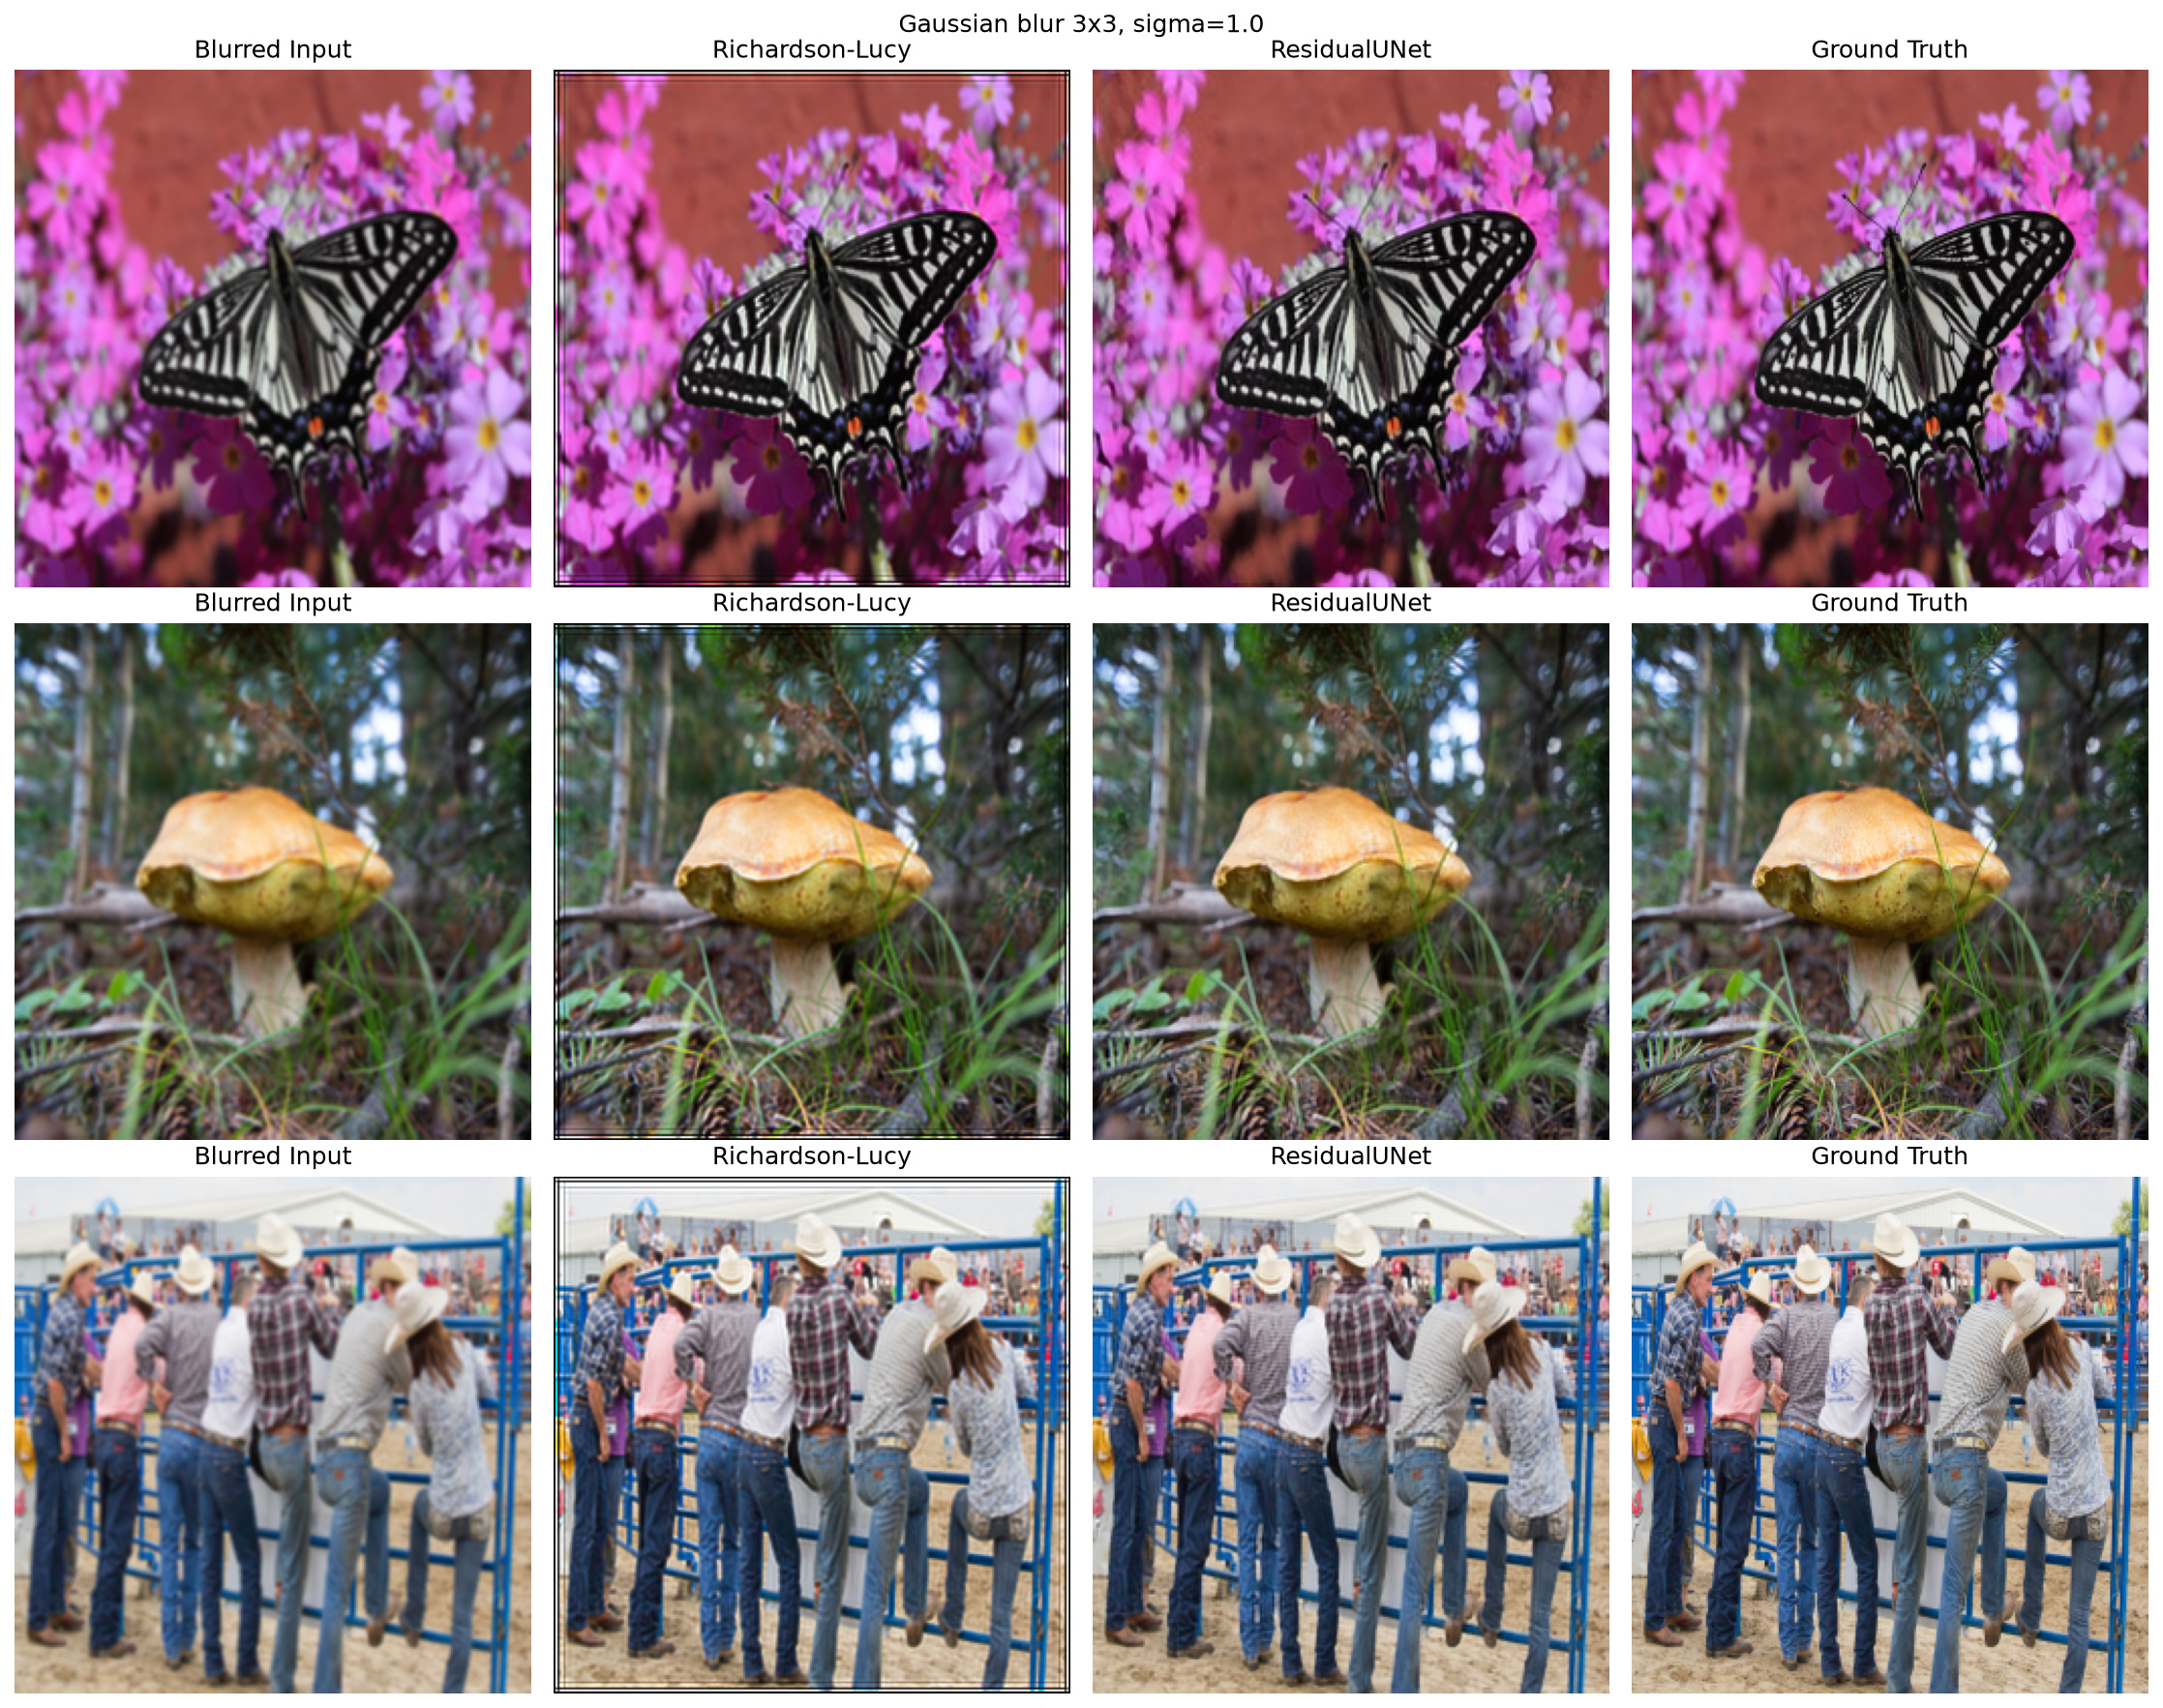
\includegraphics[width=0.67\linewidth]{images/deblurring_display/examples_k3_s1.0.jpg}\par
{\footnotesize Przykład \ensuremath{\sigma}=1.0, jądro 3x3}
\end{center}
\end{minipage}\par\vspace{5pt}
\noindent\begin{minipage}{\linewidth}
\deblurexperiment{Eksperyment: \ensuremath{\sigma} = 1.5 (rozmycie silniejsze niż treningowe)}
\begin{center}
\begin{tabular}{@{}lrrr@{}}
\toprule
Metoda & PSNR (dB) & SSIM & LPIPS \\
\midrule
Richardson-Lucy & 20.66 & 0.897 & 0.231 \\
Sieć neuronowa & 26.49 & 0.854 & 0.052 \\
\bottomrule
\end{tabular}
\end{center}
\begin{center}
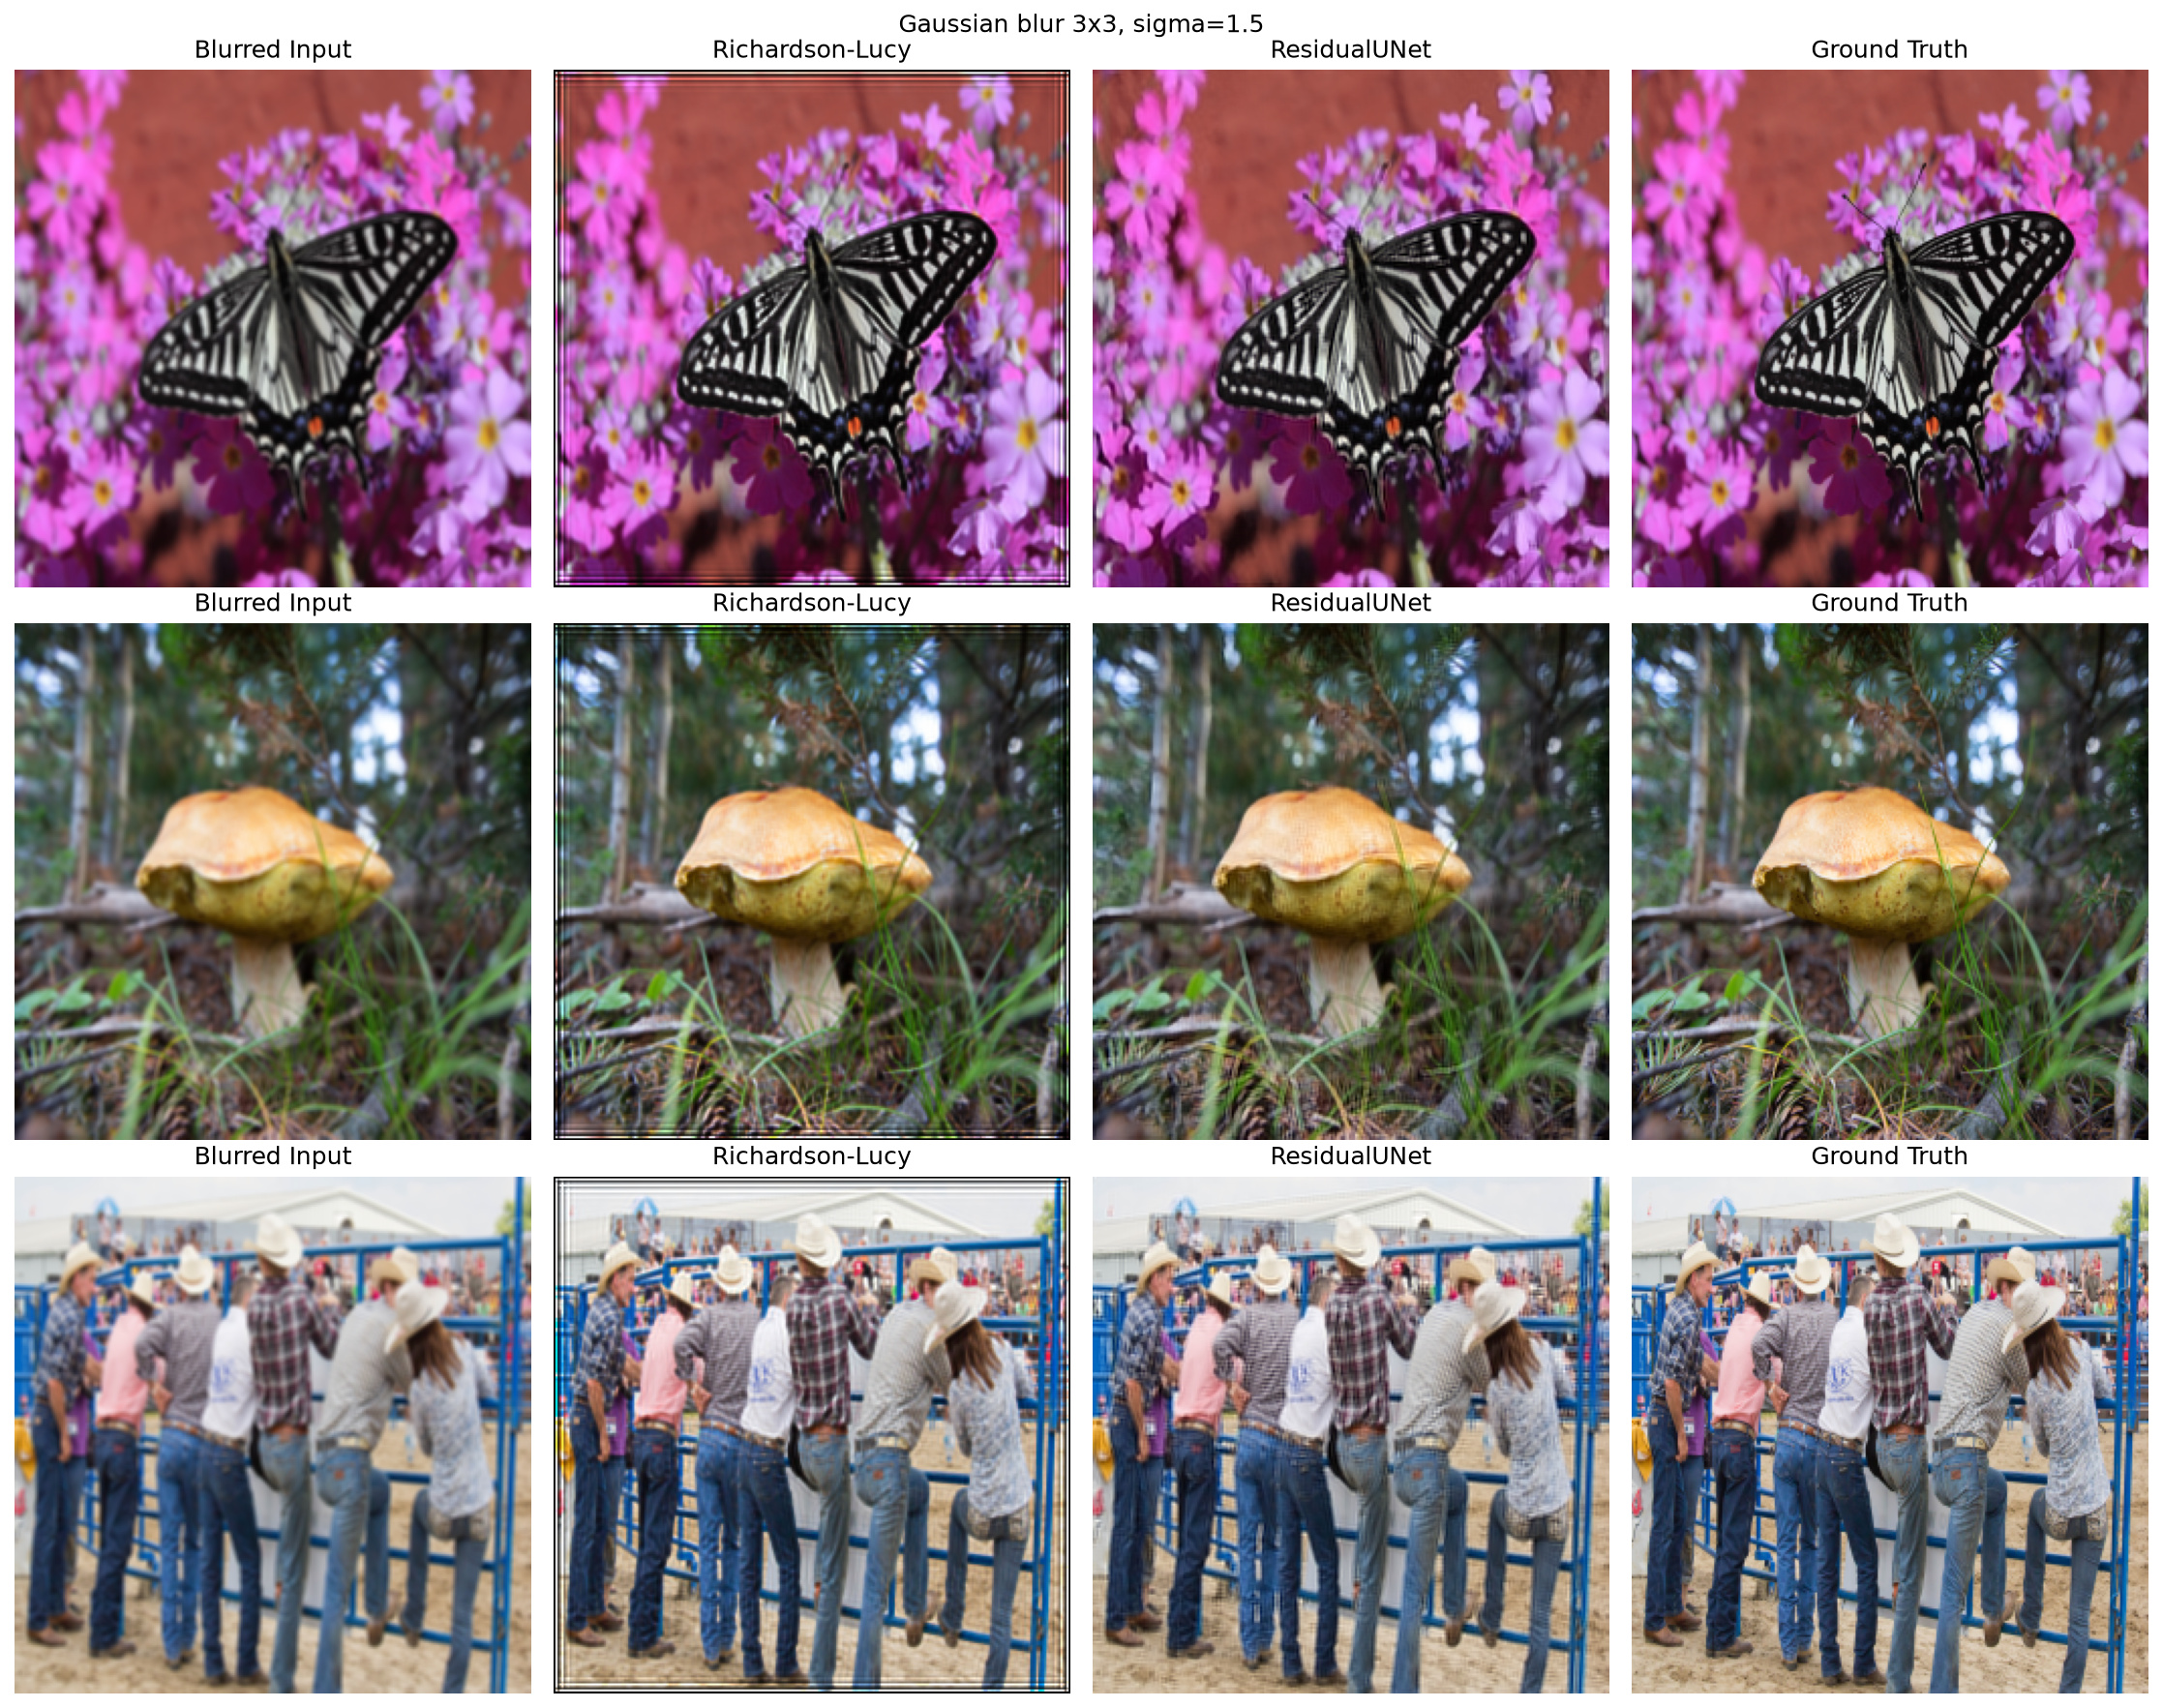
\includegraphics[width=0.67\linewidth]{images/deblurring_display/examples_k3_s1.5.jpg}\par
{\footnotesize Przykład \ensuremath{\sigma}=1.5, jądro 3x3}
\end{center}
\end{minipage}\par\vspace{5pt}
\noindent\begin{minipage}{\linewidth}
\deblurexperiment{Eksperyment: \ensuremath{\sigma} = 2.0 (rozmycie silniejsze niż treningowe)}
\begin{center}
\begin{tabular}{@{}lrrr@{}}
\toprule
Metoda & PSNR (dB) & SSIM & LPIPS \\
\midrule
Richardson-Lucy & 20.66 & 0.894 & 0.233 \\
Sieć neuronowa & 25.47 & 0.822 & 0.051 \\
\bottomrule
\end{tabular}
\end{center}
\begin{center}
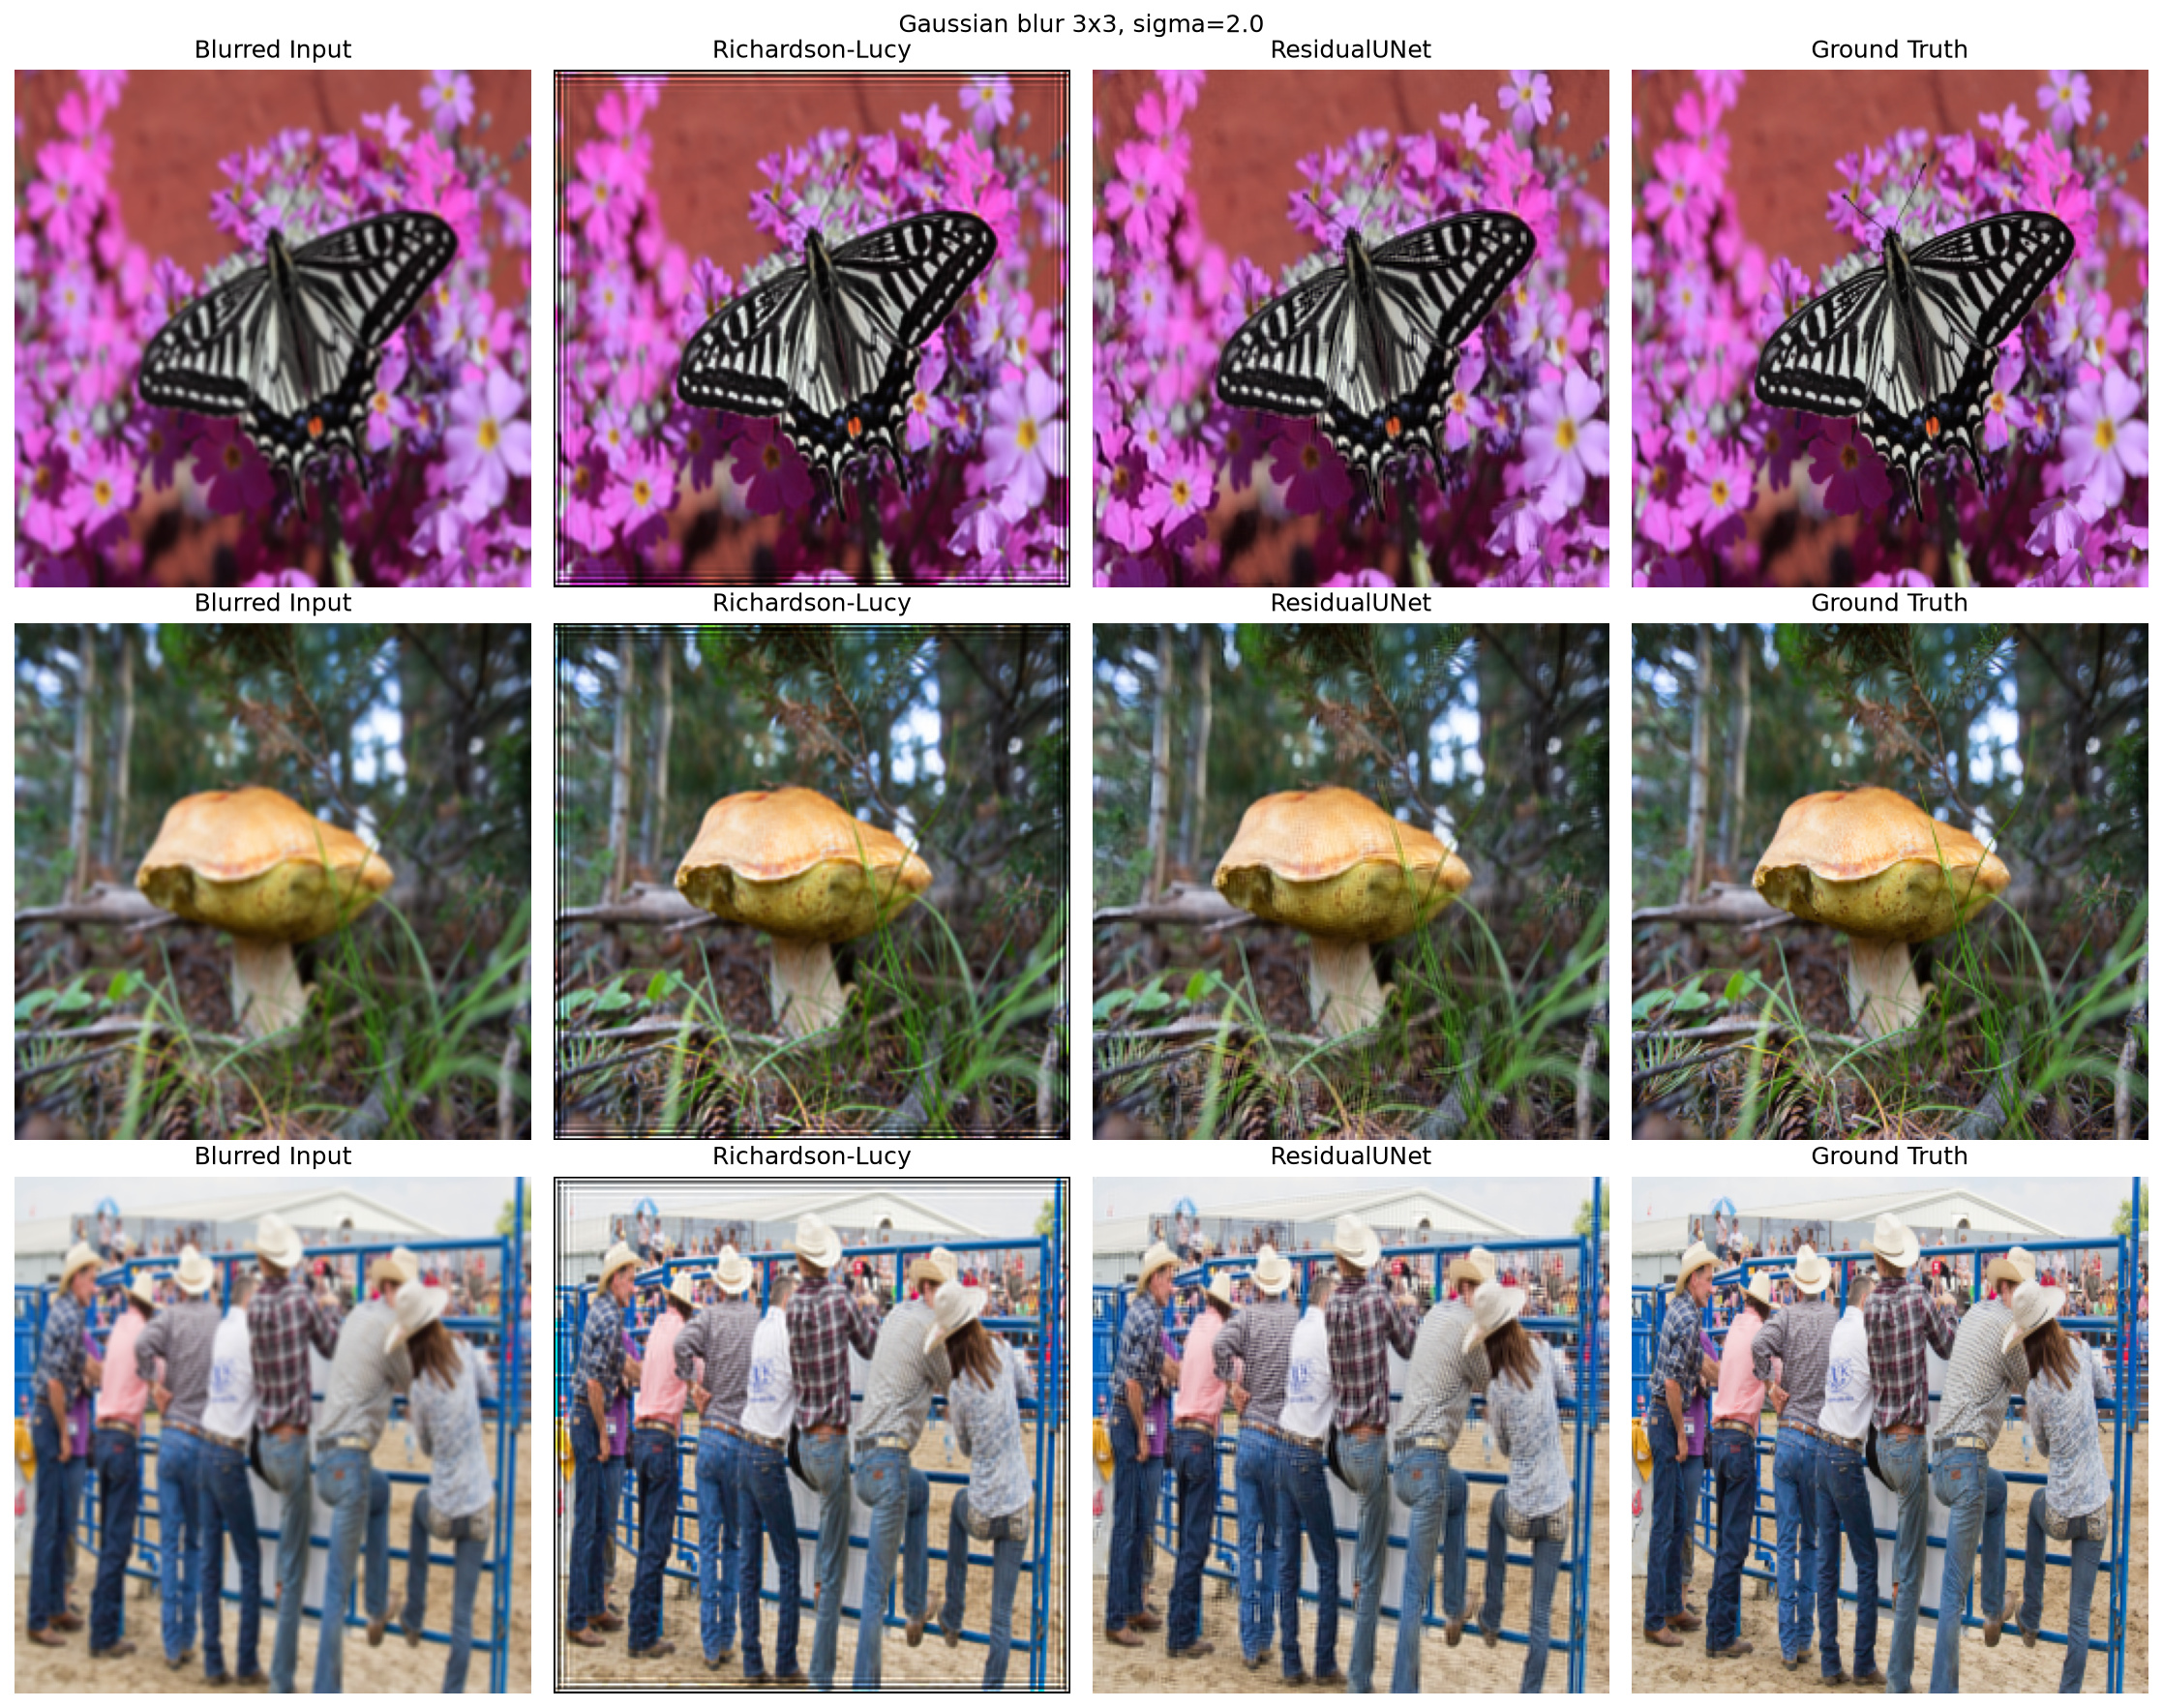
\includegraphics[width=0.67\linewidth]{images/deblurring_display/examples_k3_s2.0.jpg}\par
{\footnotesize Przykład \ensuremath{\sigma}=2.0, jądro 3x3}
\end{center}
\end{minipage}\par\vspace{5pt}
\subsubsection*{3.2 Jądro rozmycia 5x5}
\noindent\begin{minipage}{\linewidth}
\deblurexperiment{Eksperyment: \ensuremath{\sigma} = 0.8 (rozmycie słabsze niż treningowe)}
\begin{center}
\begin{tabular}{@{}lrrr@{}}
\toprule
Metoda & PSNR (dB) & SSIM & LPIPS \\
\midrule
Richardson-Lucy & 23.96 & 0.941 & 0.104 \\
Sieć neuronowa & 34.10 & 0.974 & 0.010 \\
\bottomrule
\end{tabular}
\end{center}
\begin{center}
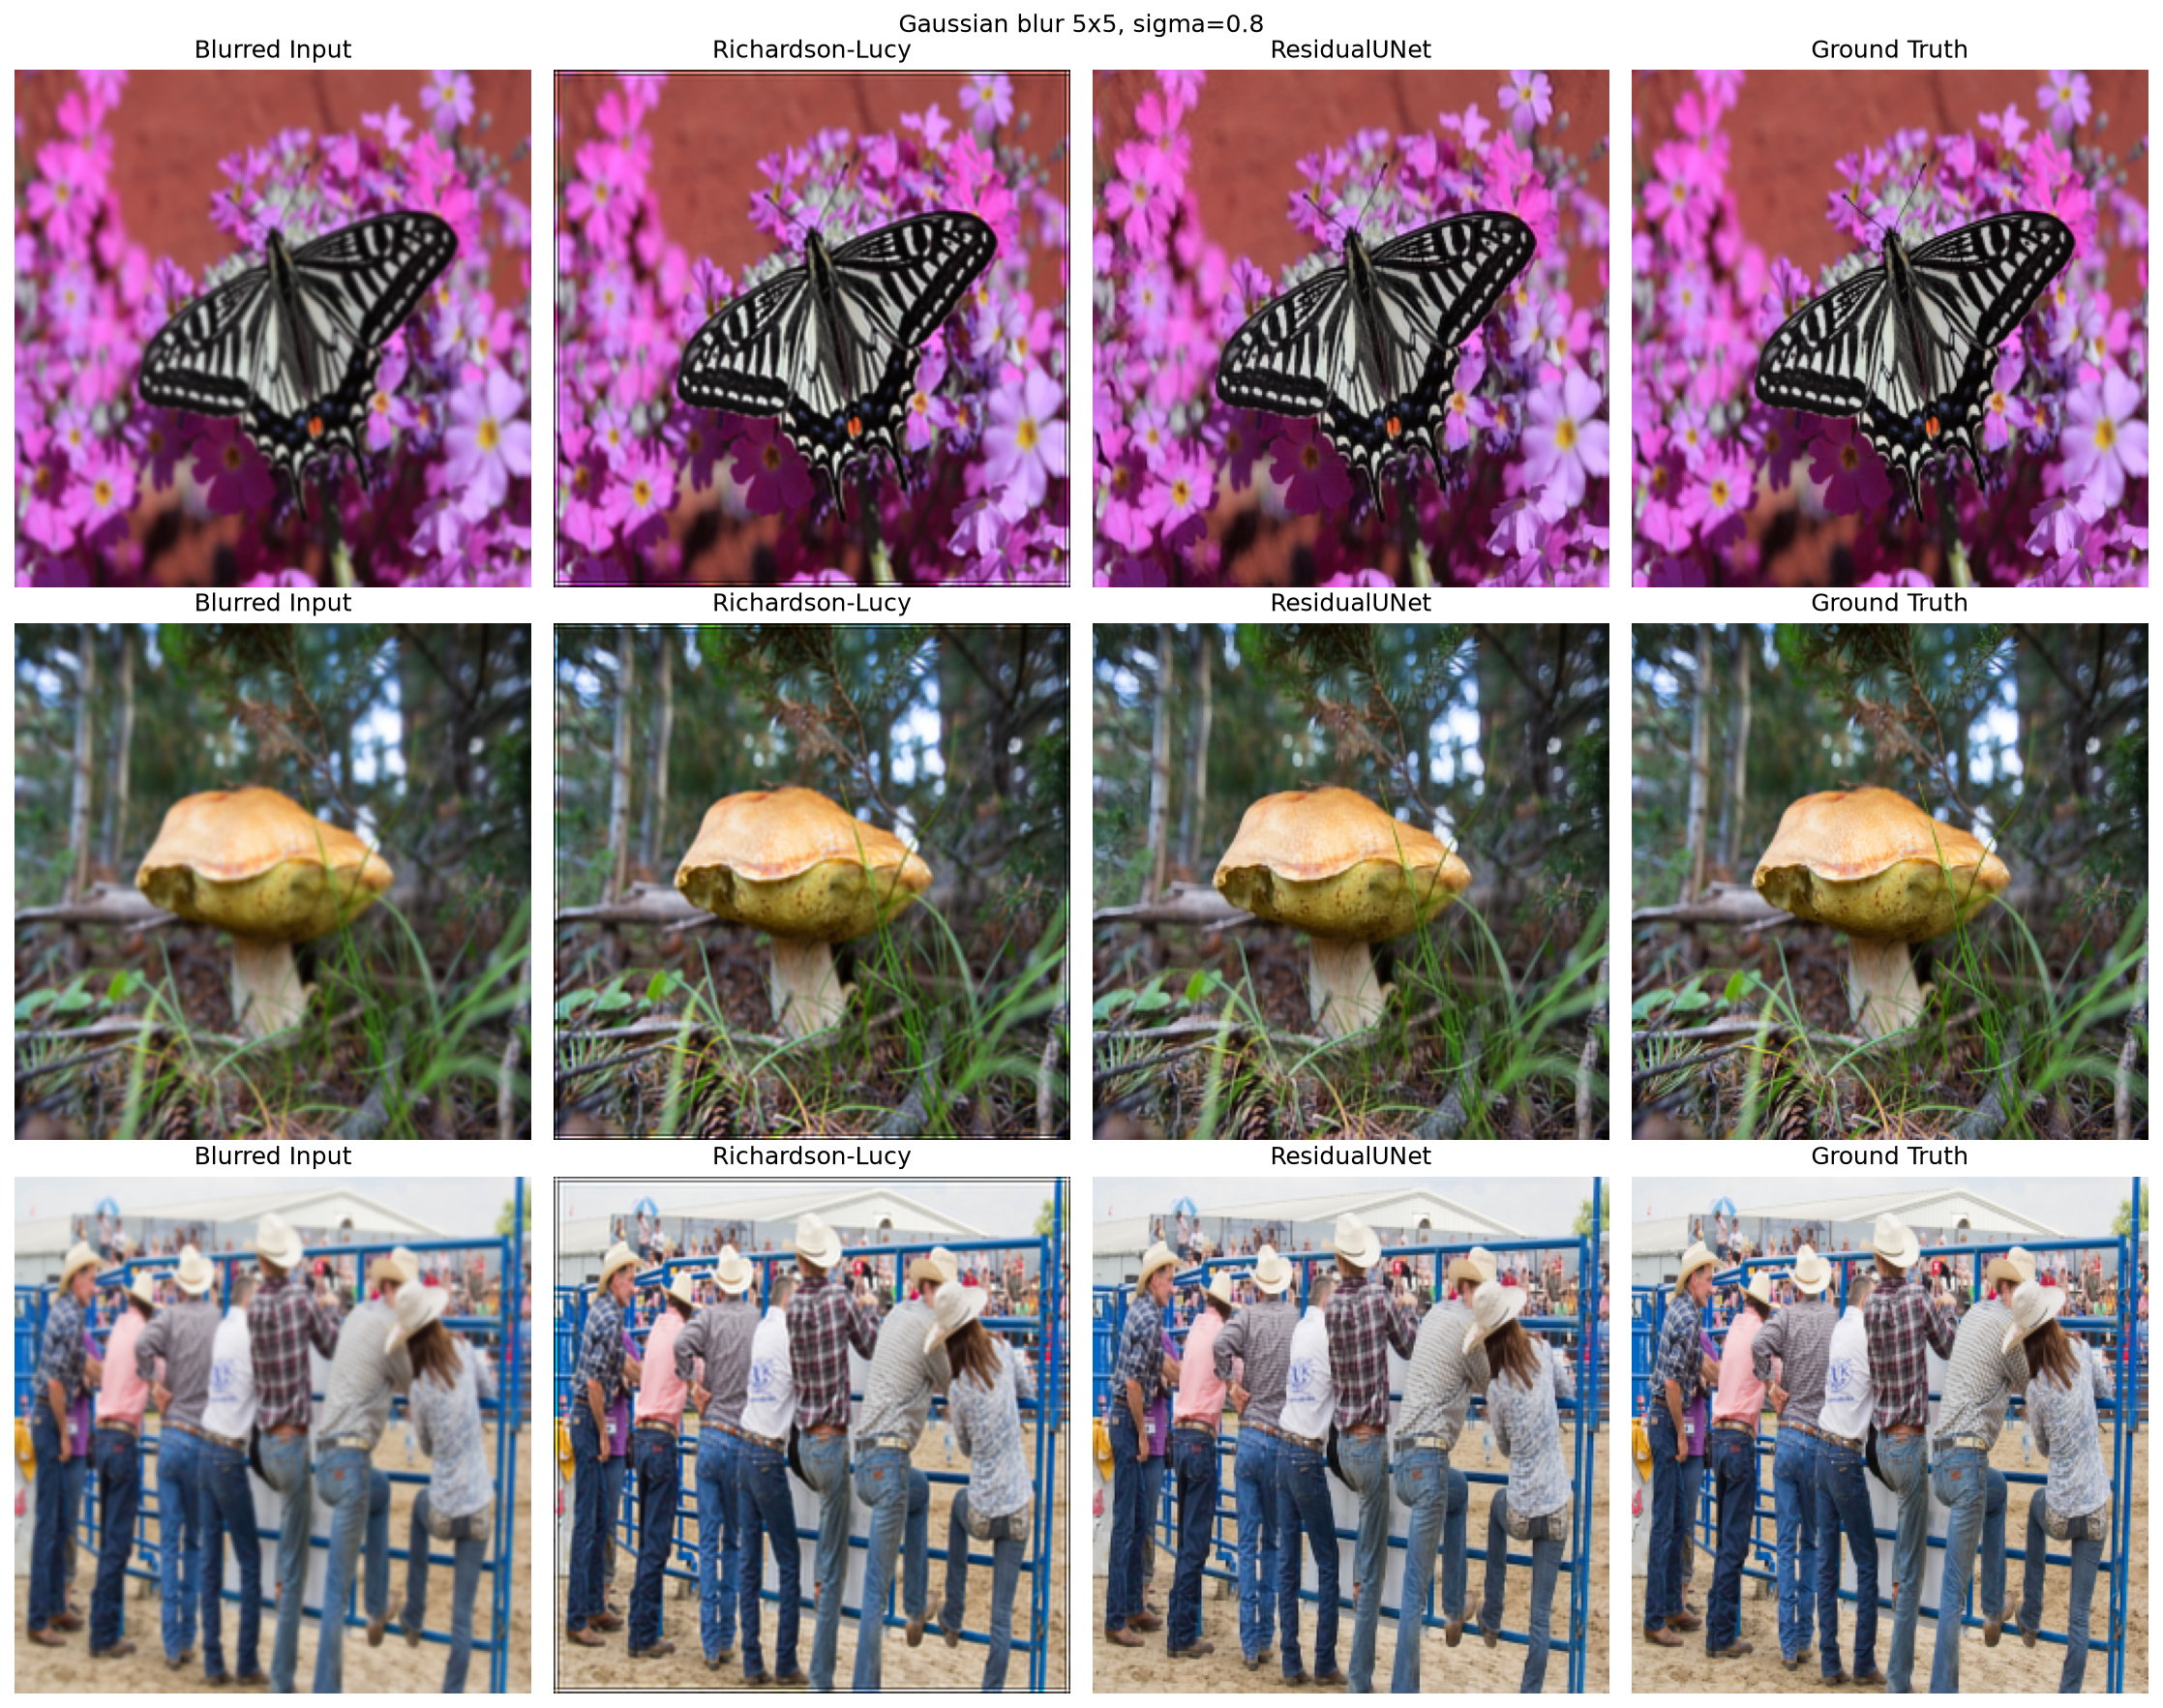
\includegraphics[width=0.67\linewidth]{images/deblurring_display/examples_k5_s0.8.jpg}\par
{\footnotesize Przykład \ensuremath{\sigma}=0.8, jądro 5x5}
\end{center}
\end{minipage}\par\vspace{5pt}
\noindent\begin{minipage}{\linewidth}
\deblurexperiment{Eksperyment: \ensuremath{\sigma} = 1.0 (rozmycie słabsze niż treningowe)}
\begin{center}
\begin{tabular}{@{}lrrr@{}}
\toprule
Metoda & PSNR (dB) & SSIM & LPIPS \\
\midrule
Richardson-Lucy & 21.72 & 0.896 & 0.227 \\
Sieć neuronowa & 29.64 & 0.929 & 0.085 \\
\bottomrule
\end{tabular}
\end{center}
\begin{center}
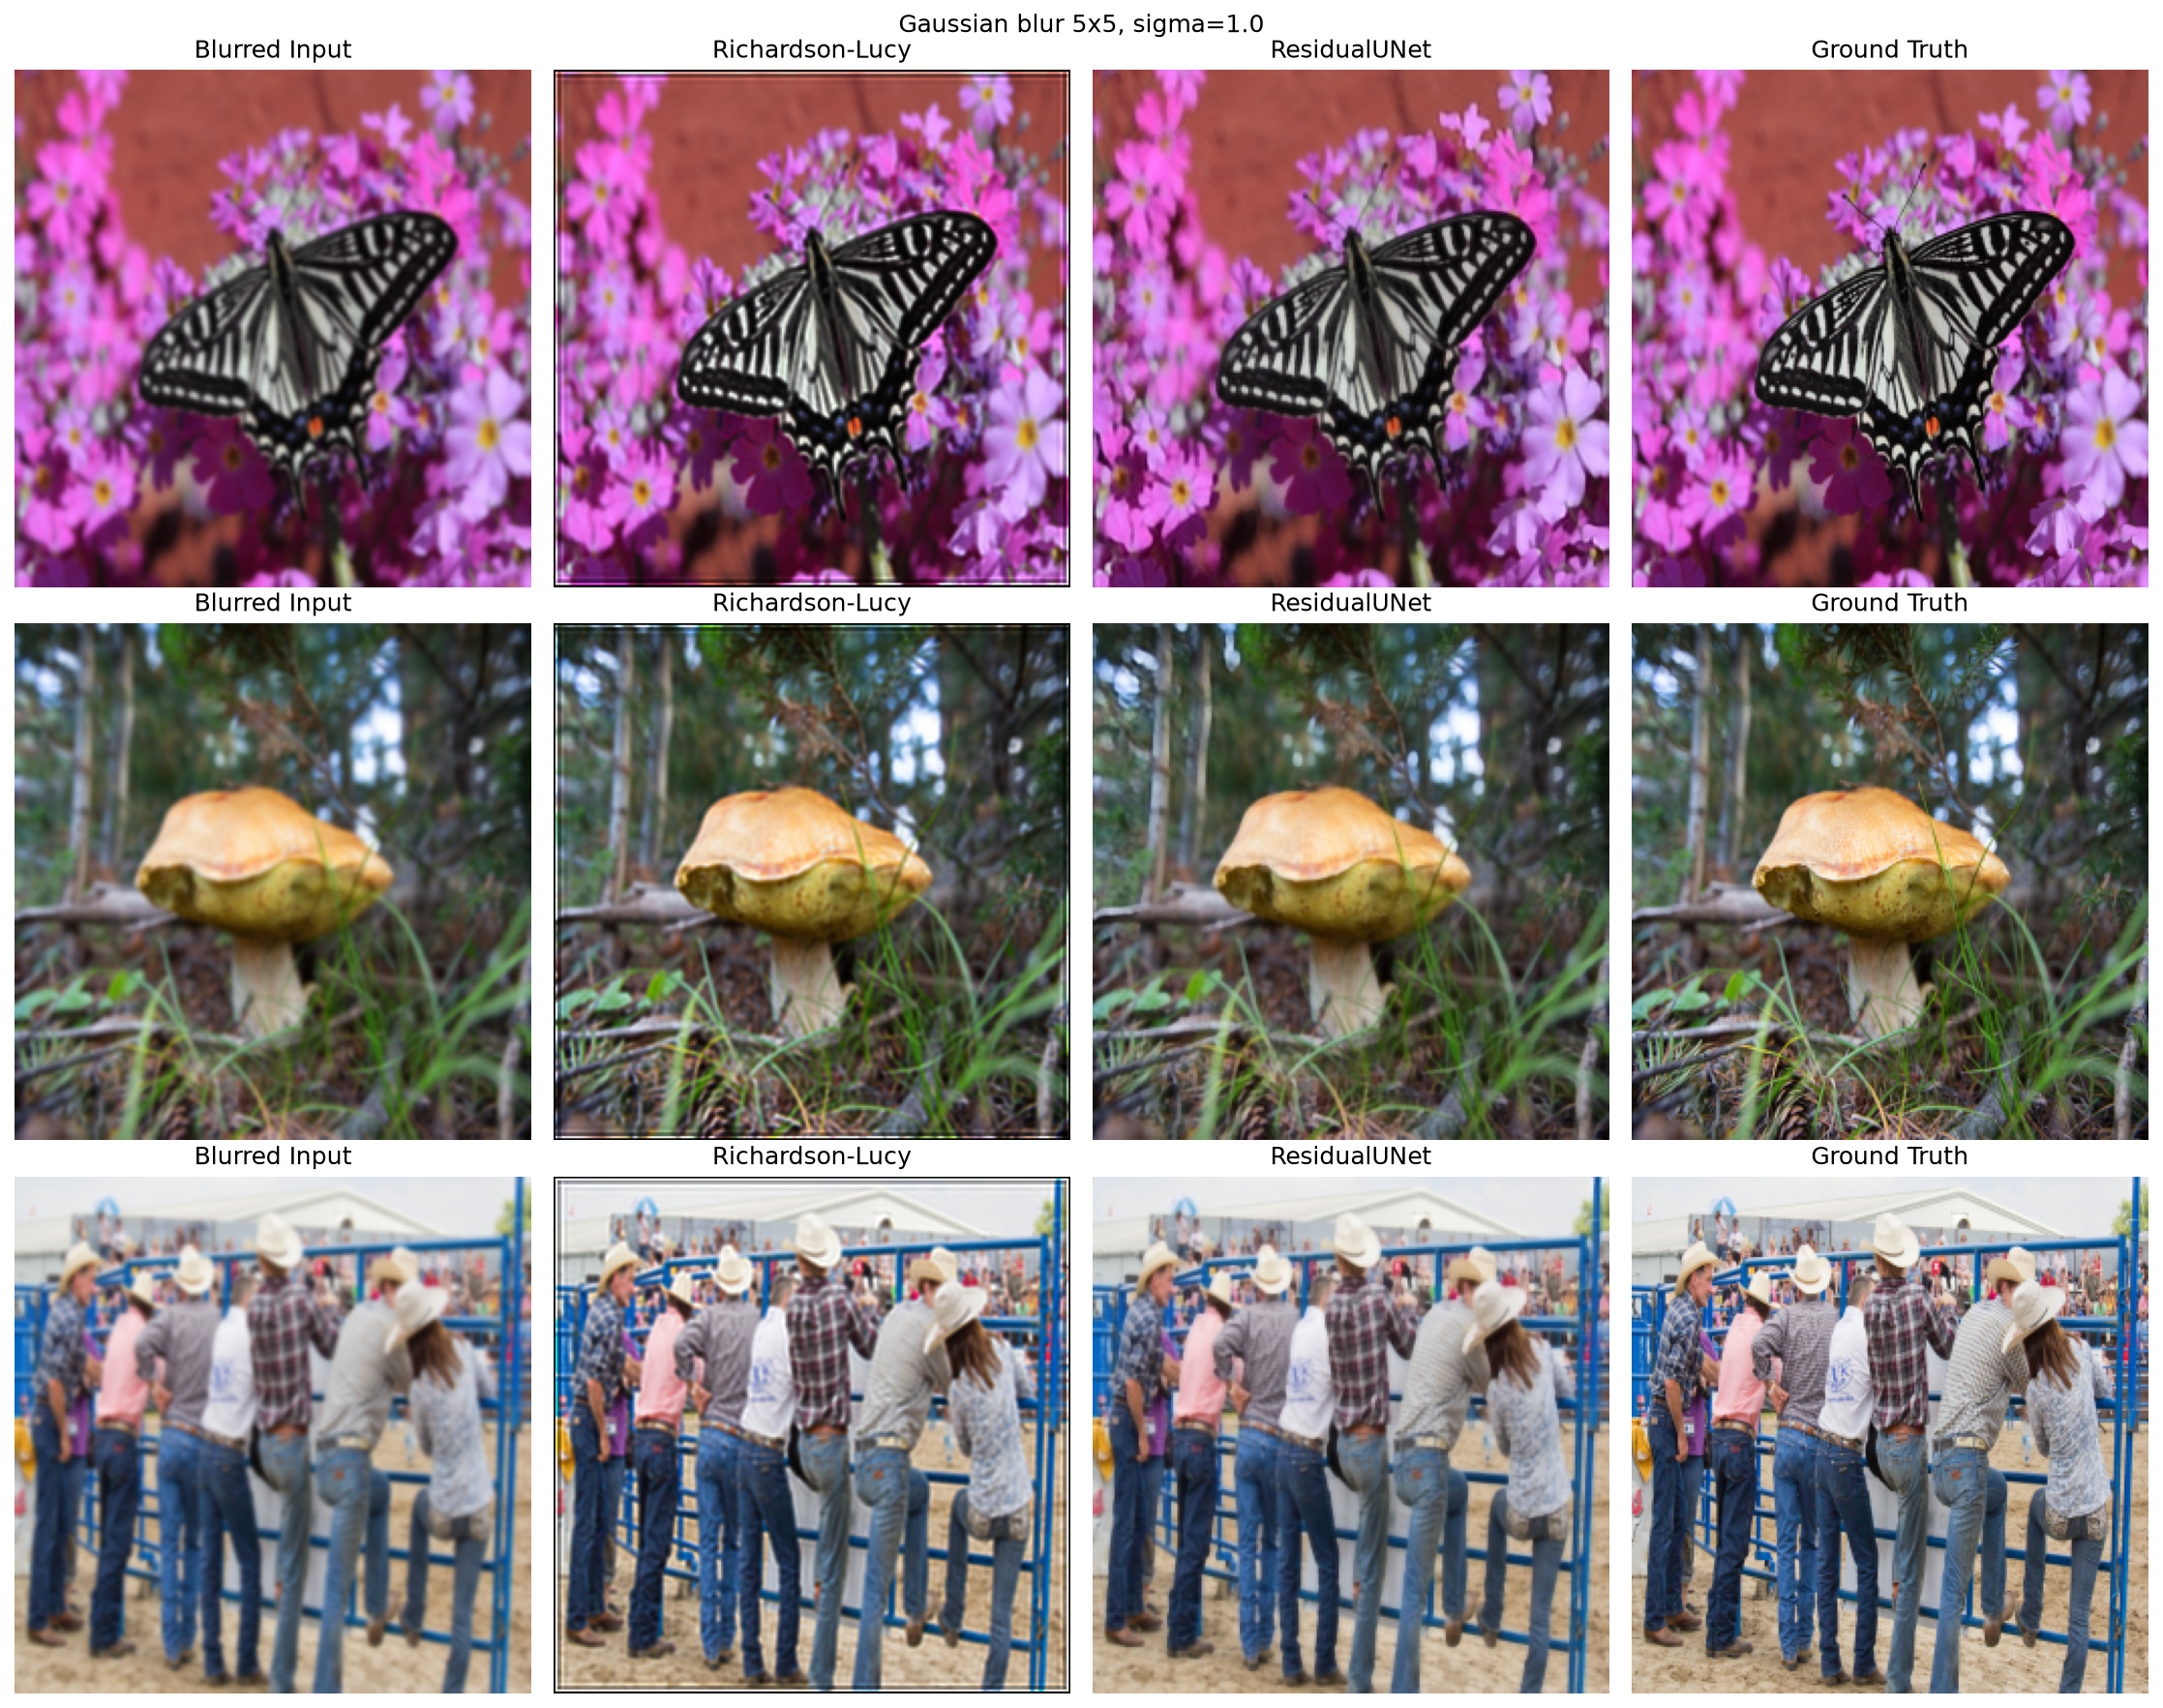
\includegraphics[width=0.67\linewidth]{images/deblurring_display/examples_k5_s1.0.jpg}\par
{\footnotesize Przykład \ensuremath{\sigma}=1.0, jądro 5x5}
\end{center}
\end{minipage}\par\vspace{5pt}
\noindent\begin{minipage}{\linewidth}
\deblurexperiment{Eksperyment: \ensuremath{\sigma} = 1.5 (siła rozmycia użyta w treningu)}
\begin{center}
\begin{tabular}{@{}lrrr@{}}
\toprule
Metoda & PSNR (dB) & SSIM & LPIPS \\
\midrule
Richardson-Lucy & 19.93 & 0.812 & 0.372 \\
Sieć neuronowa & 26.75 & 0.857 & 0.132 \\
\bottomrule
\end{tabular}
\end{center}
\begin{center}
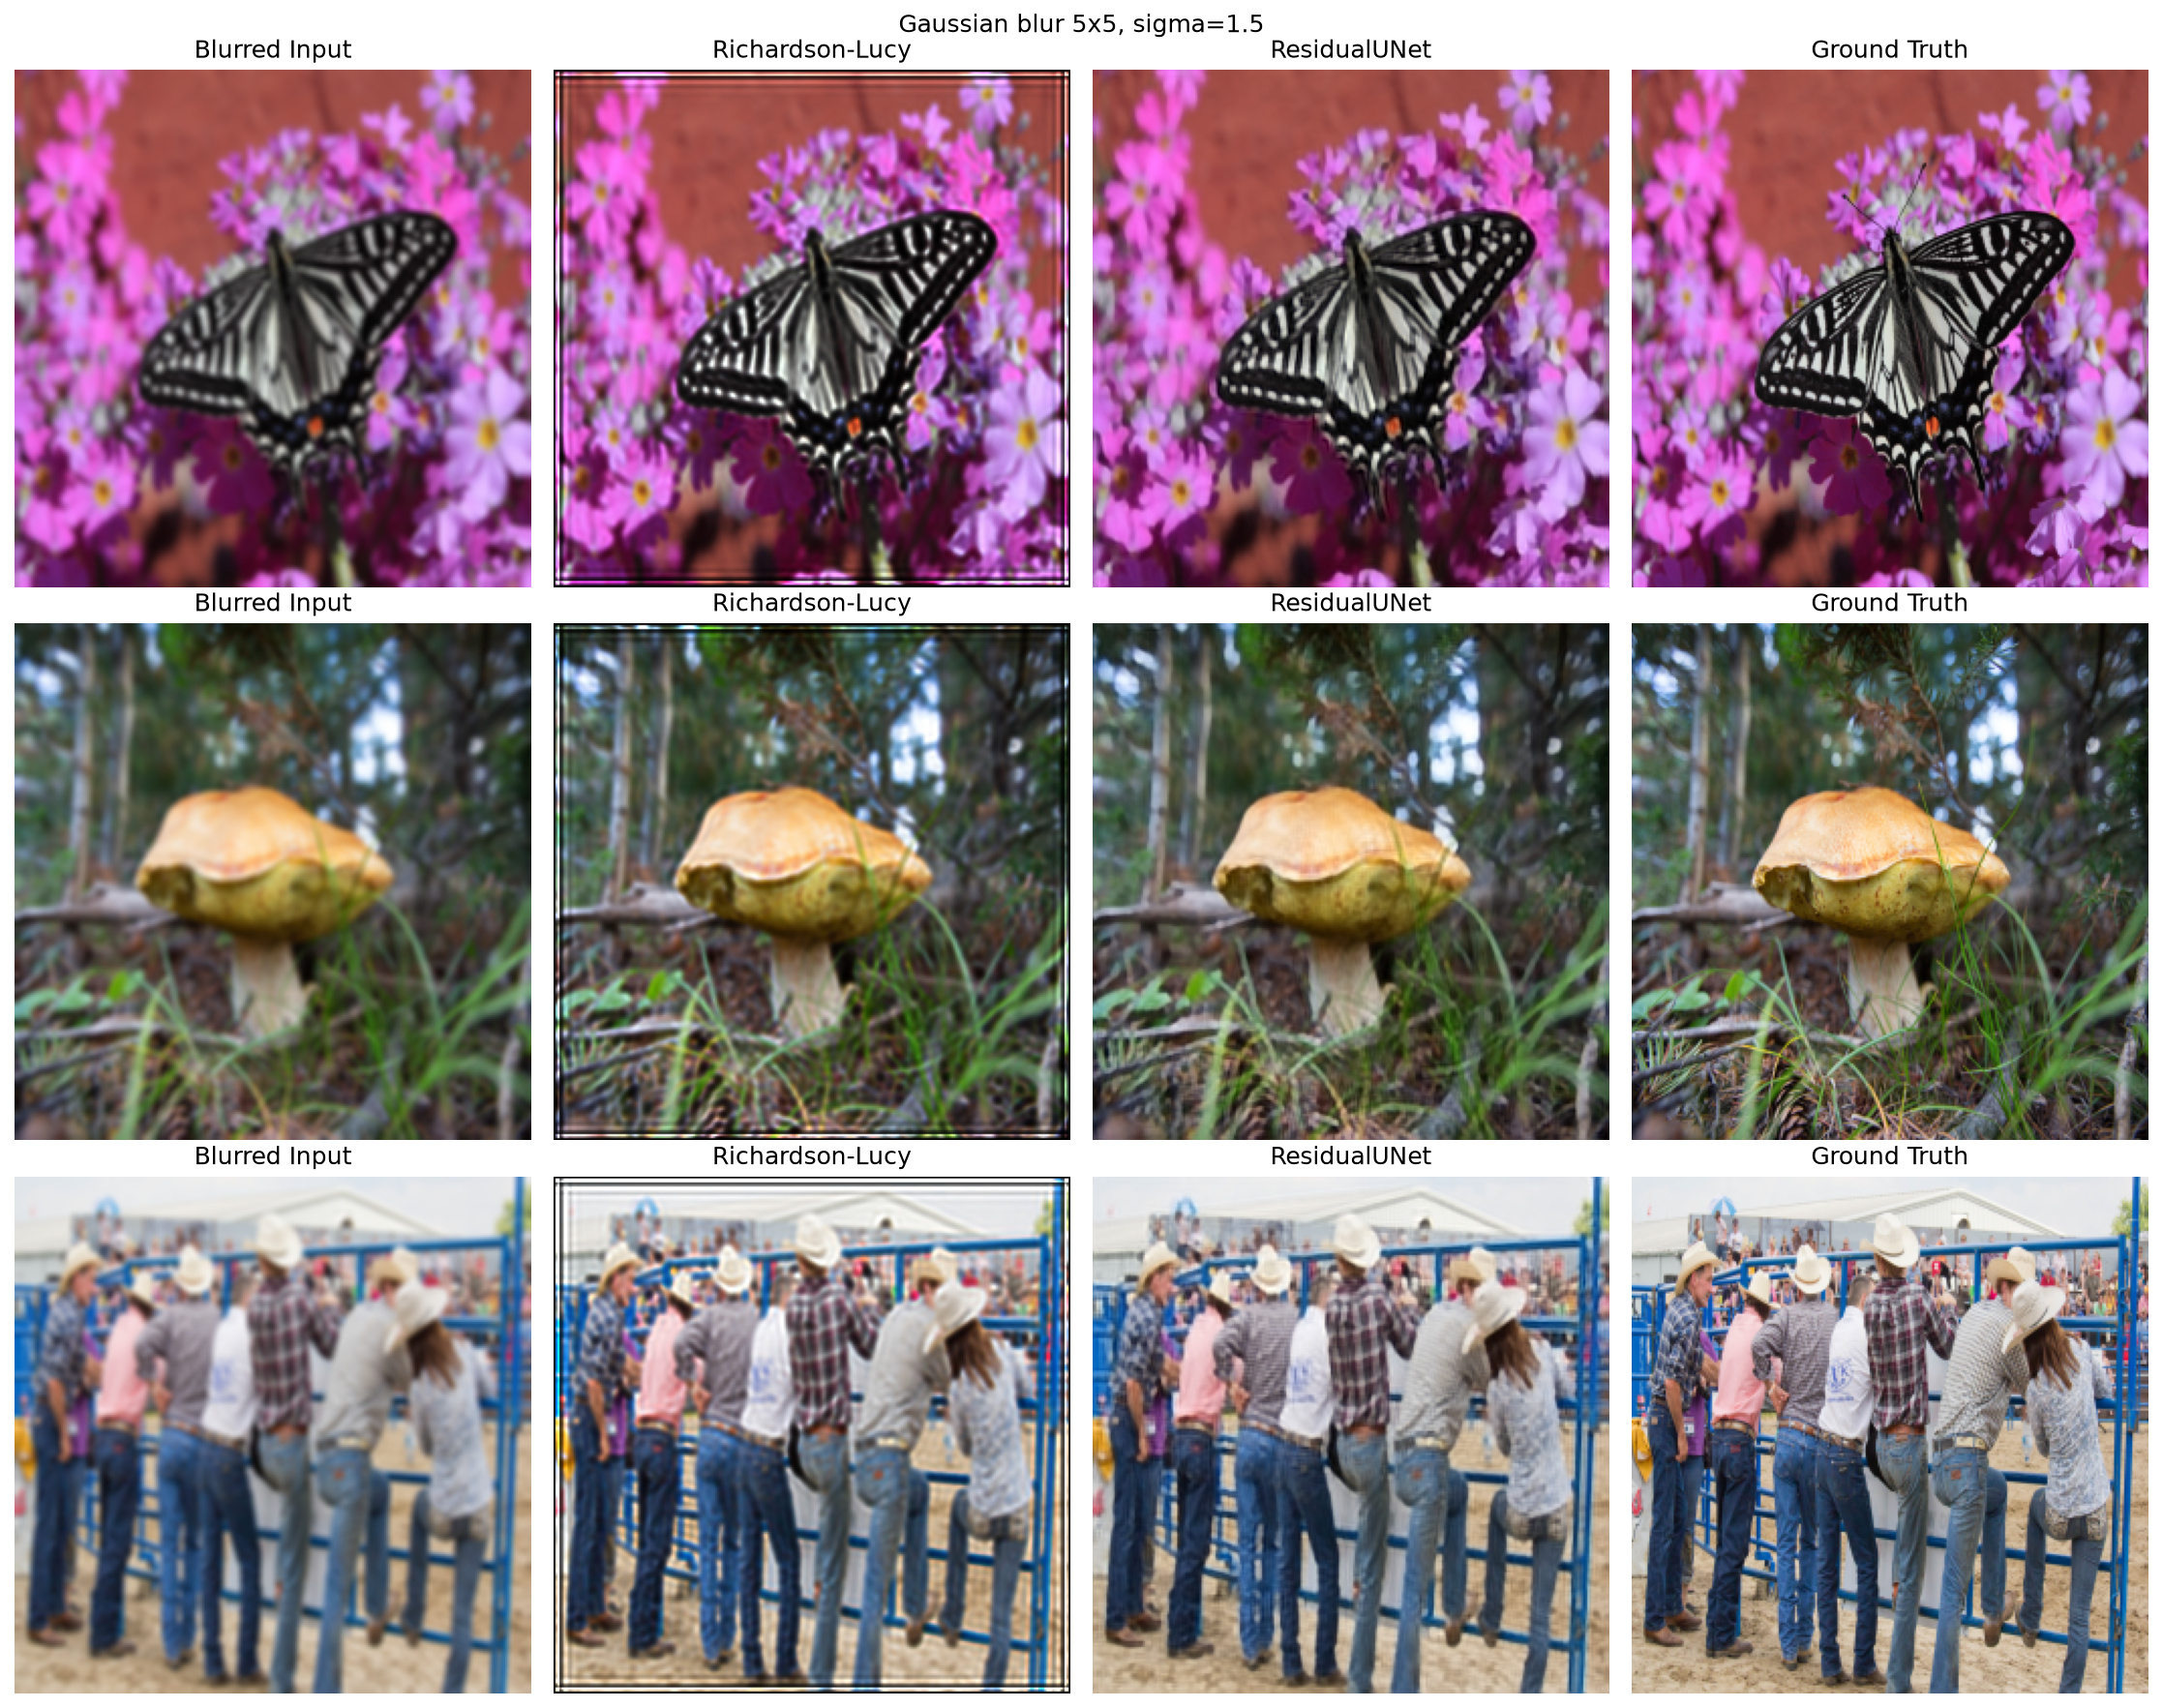
\includegraphics[width=0.67\linewidth]{images/deblurring_display/examples_k5_s1.5.jpg}\par
{\footnotesize Przykład \ensuremath{\sigma}=1.5, jądro 5x5}
\end{center}
\end{minipage}\par\vspace{5pt}
\noindent\begin{minipage}{\linewidth}
\deblurexperiment{Eksperyment: \ensuremath{\sigma} = 2.0 (rozmycie silniejsze niż treningowe)}
\begin{center}
\begin{tabular}{@{}lrrr@{}}
\toprule
Metoda & PSNR (dB) & SSIM & LPIPS \\
\midrule
Richardson-Lucy & 18.50 & 0.785 & 0.374 \\
Sieć neuronowa & 24.49 & 0.768 & 0.115 \\
\bottomrule
\end{tabular}
\end{center}
\begin{center}
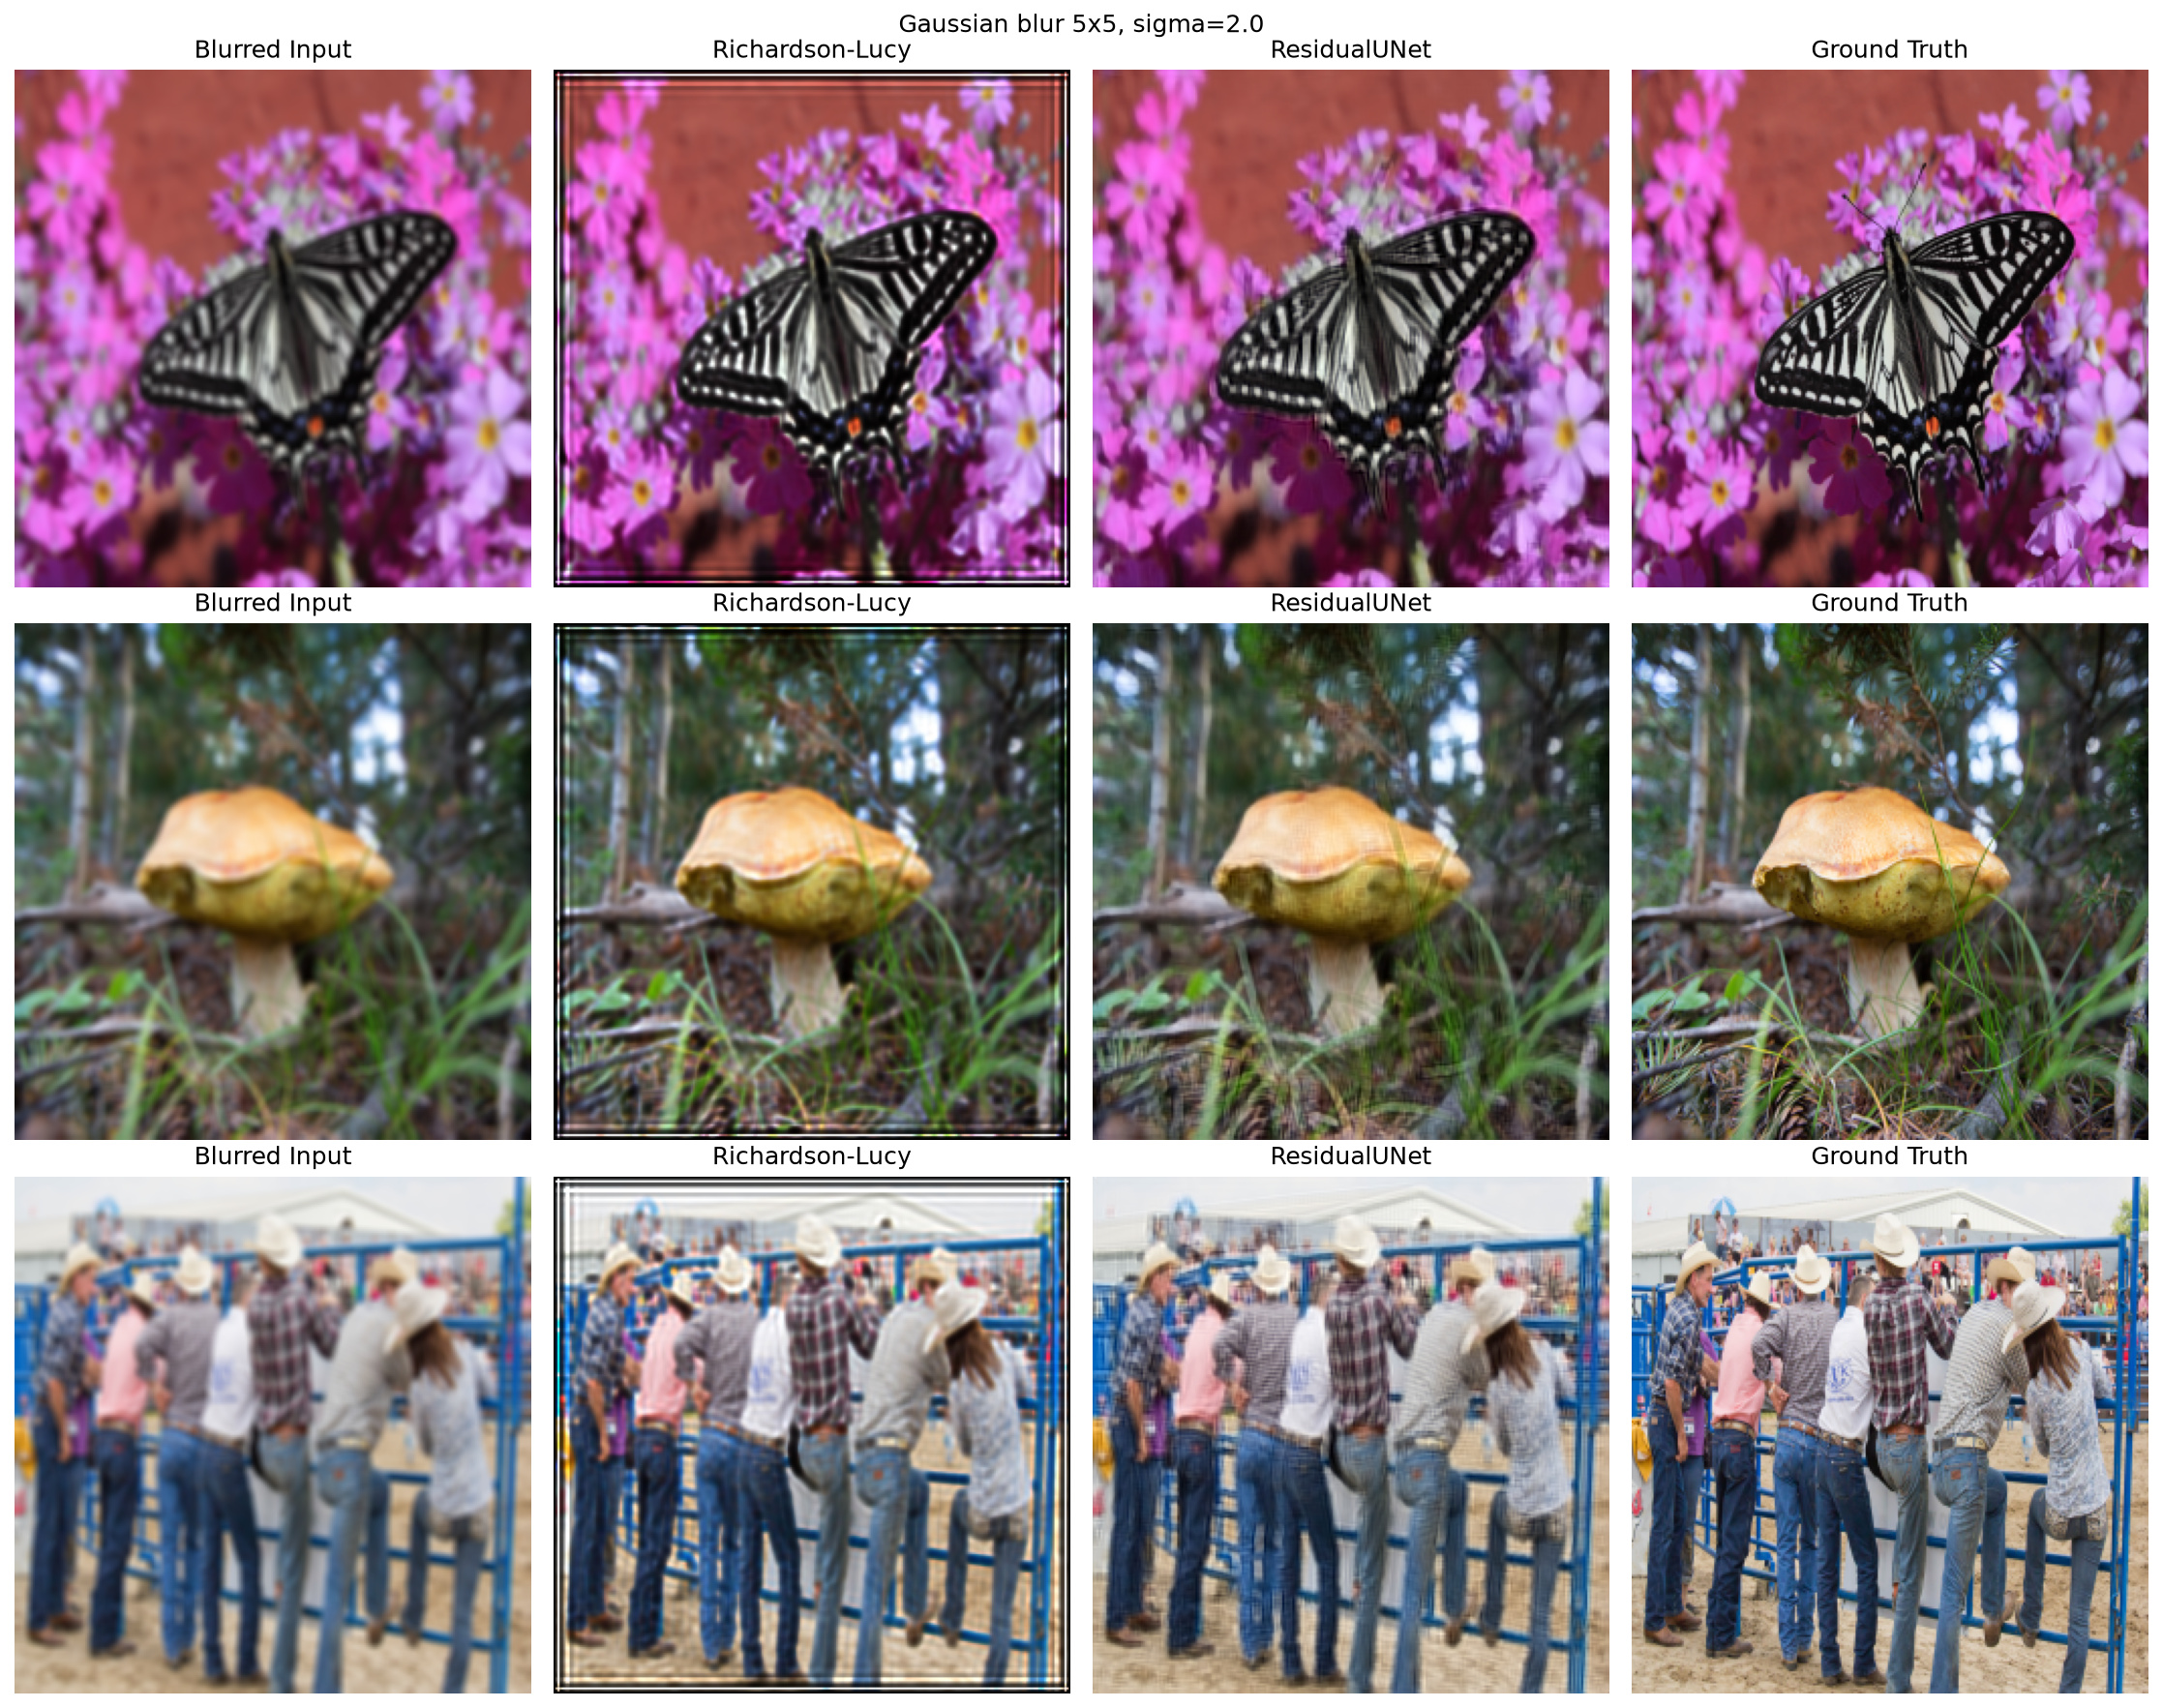
\includegraphics[width=0.67\linewidth]{images/deblurring_display/examples_k5_s2.0.jpg}\par
{\footnotesize Przykład \ensuremath{\sigma}=2.0, jądro 5x5}
\end{center}
\end{minipage}\par\vspace{5pt}
\noindent\begin{minipage}{\linewidth}
\deblurexperiment{Eksperyment: \ensuremath{\sigma} = 3.0 (rozmycie znacznie silniejsze niż treningowe)}
\begin{center}
\begin{tabular}{@{}lrrr@{}}
\toprule
Metoda & PSNR (dB) & SSIM & LPIPS \\
\midrule
Richardson-Lucy & 18.06 & 0.774 & 0.349 \\
Sieć neuronowa & 23.10 & 0.695 & 0.164 \\
\bottomrule
\end{tabular}
\end{center}
\begin{center}
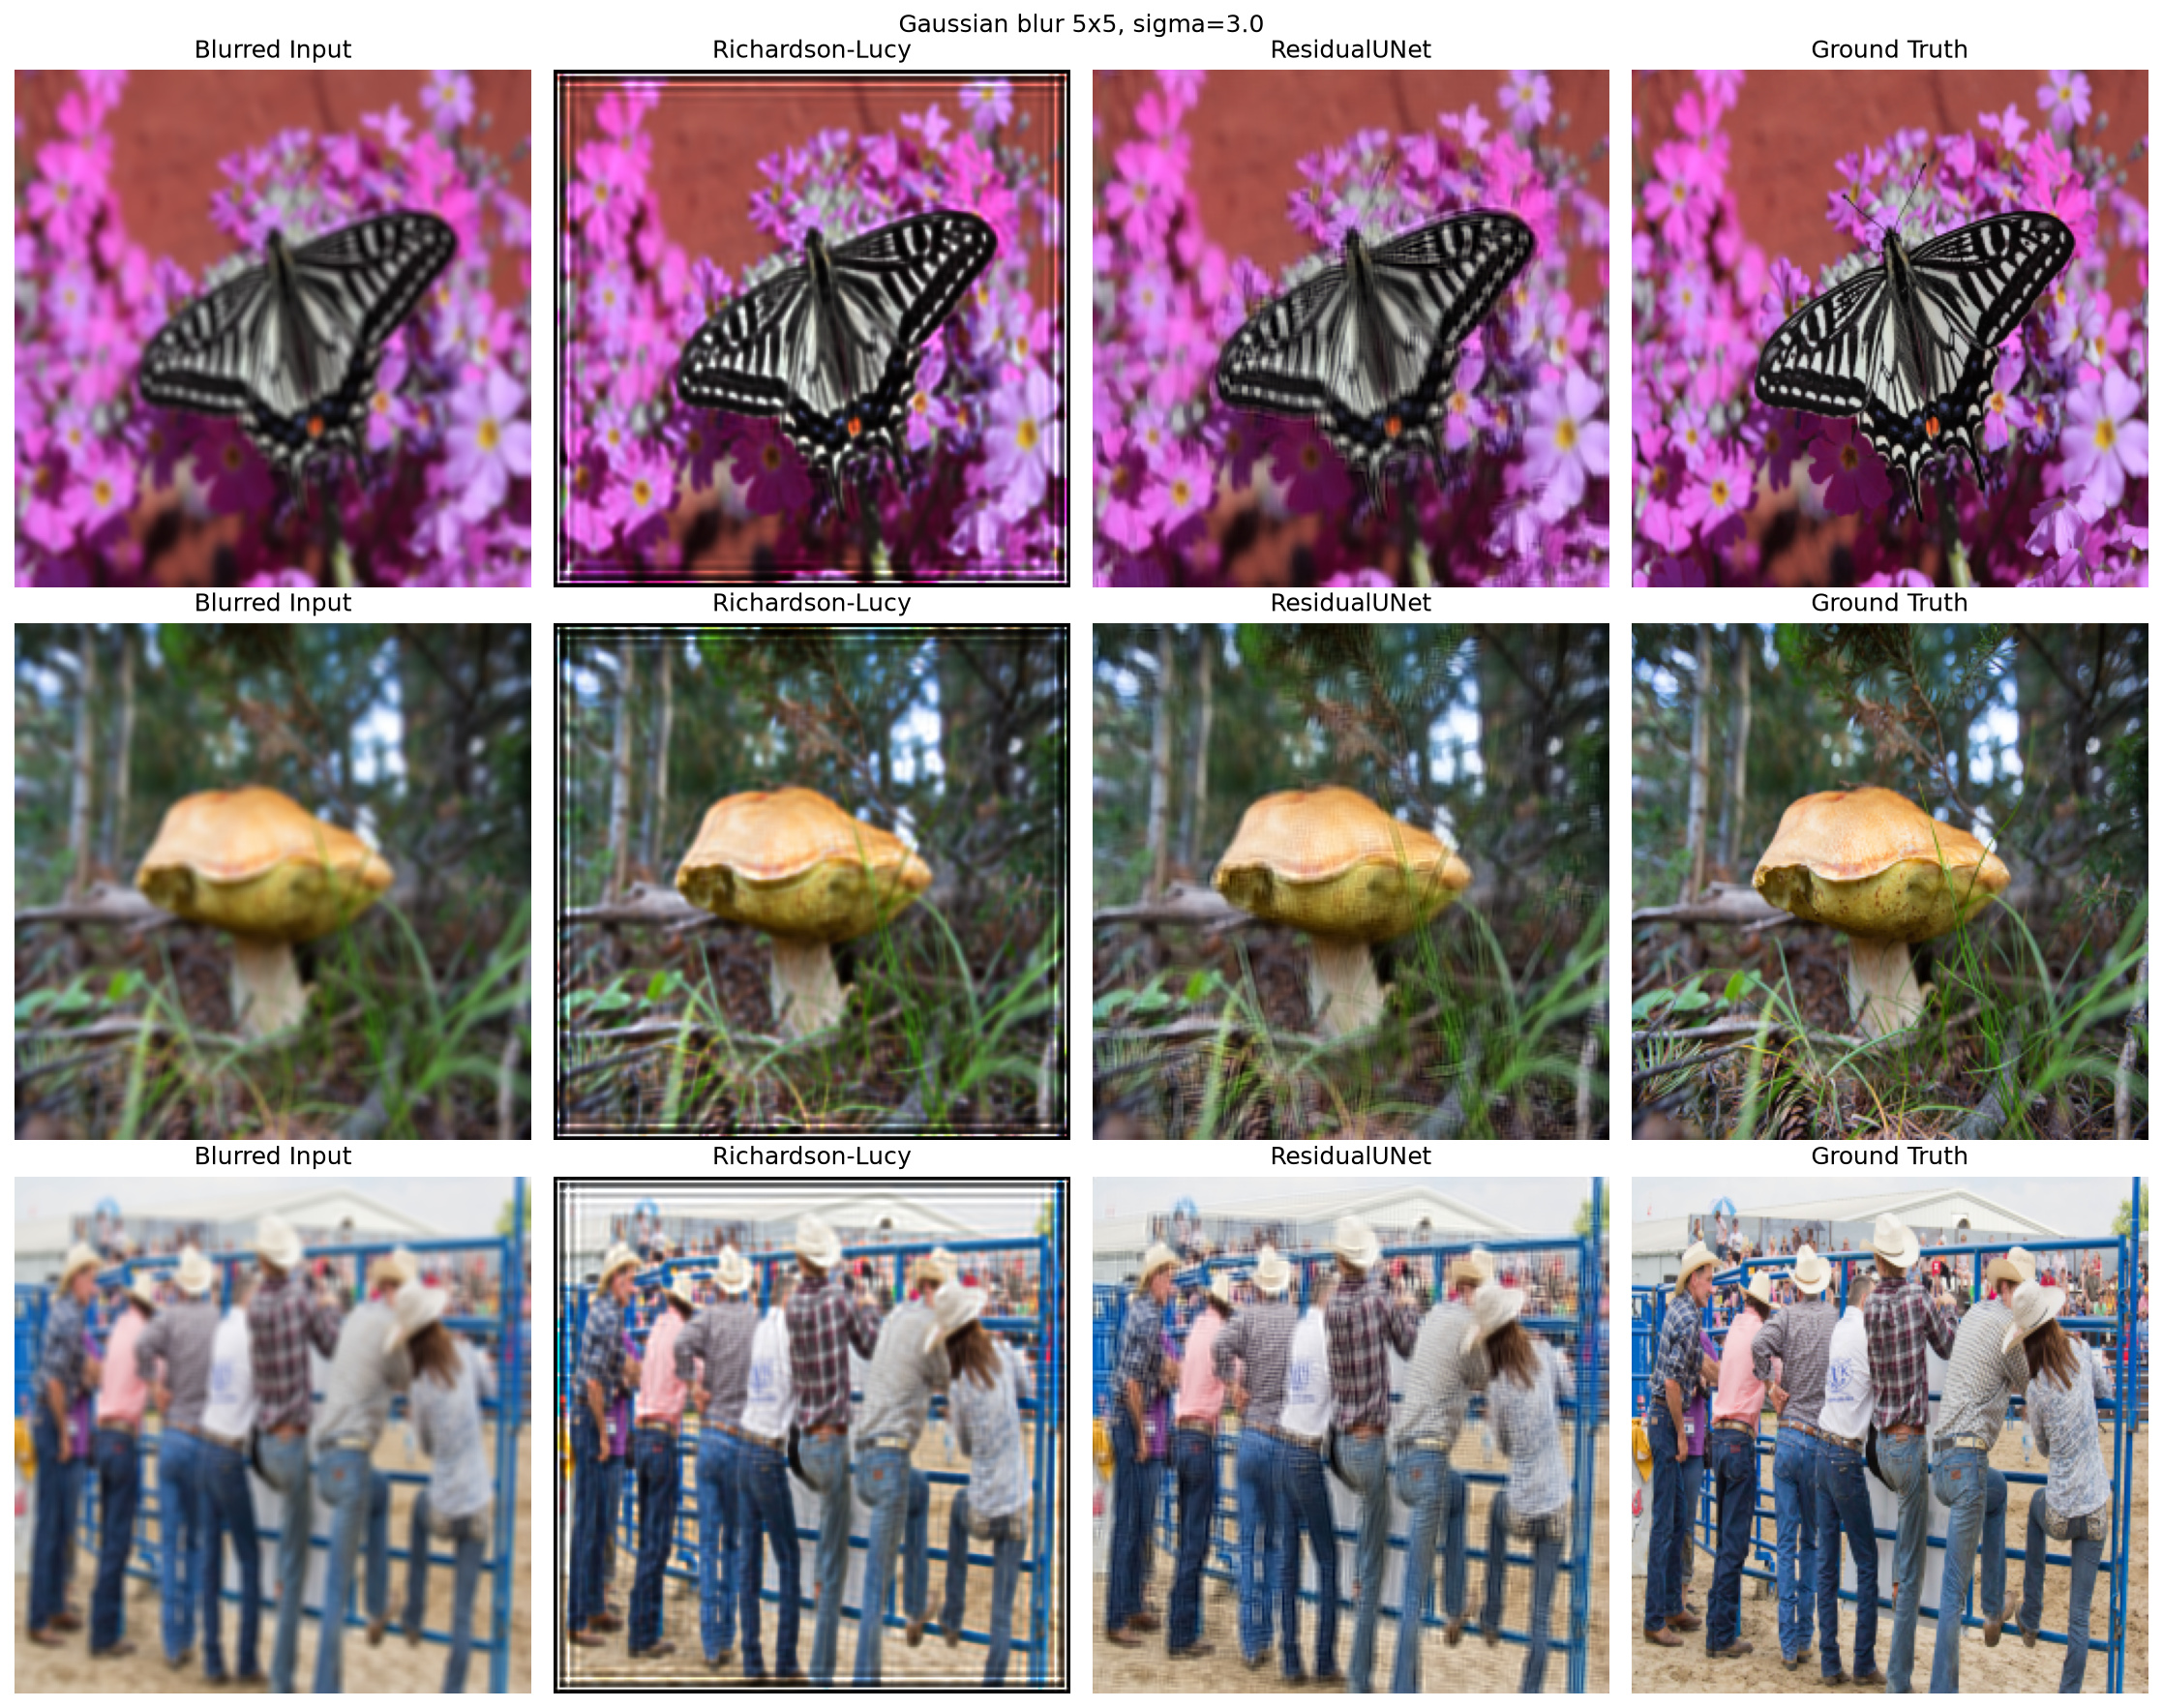
\includegraphics[width=0.67\linewidth]{images/deblurring_display/examples_k5_s3.0.jpg}\par
{\footnotesize Przykład \ensuremath{\sigma}=3.0, jądro 5x5}
\end{center}
\end{minipage}\par\vspace{5pt}
\subsection*{4. Wnioski}
\begin{itemize}
\item Dla rozmycia o sile zbliżonej do treningowej lub silniejszej (\ensuremath{\sigma} \ensuremath{\geq} 0.8) sieć neuronowa wyraźnie przewyższa metodę klasyczną we wszystkich trzech metrykach, a różnica w LPIPS jest szczególnie duża --- obrazy wyglądają percepcyjnie dużo bliżej oryginału.
\item Dla bardzo słabego rozmycia (3x3, \ensuremath{\sigma}=0.5, niemal brak rozmycia) sieć wypada gorzej niż metoda klasyczna --- nie rozpoznaje, że obraz jest już prawie ostry, i wprowadza niepotrzebne zmiany. Richardson-Lucy radzi sobie tu niemal idealnie, ponieważ zna dokładny kształt rozmycia.
\item Wraz ze wzrostem siły rozmycia powyżej wartości treningowych jakość rekonstrukcji sieci spada, jednak nadal pozostaje wyraźnie lepsza od metody klasycznej pod względem percepcyjnym (LPIPS).
\item Metoda klasyczna korzysta z dokładnie znanego kształtu rozmycia, co w praktyce rzadko jest dostępne --- mimo to przegrywa z siecią w większości testowanych przypadków, poza skrajnie słabym rozmyciem.
\end{itemize}
\endgroup

\end{document}
